% For printing in a4
%\documentclass[a4,10pt,twoside,openright,italian,english]{book}% twoside!

% For printing with the A5 format
\documentclass[11pt,twoside,openright,english,italian]{book}% twoside!

% Set paper size
\usepackage[twoside=true]{geometry}

\geometry{a4paper,
  top=33mm,
  bottom=34mm,
  inner=38mm,
  outer=32mm,
  bindingoffset=5mm
}

%\usepackage[cam,center,a4,pdflatex,axes]{crop}

\usepackage{phdthesis}
\usepackage{phdtitle}



\usepackage{listings}
\usepackage{subfig}
\usepackage{graphicx}
\usepackage{xcolor}
\usepackage{bibentry}
\usepackage{setspace}
\usepackage[english,italian]{babel}
\usepackage[toc]{appendix}
\usepackage[bookmarks=true,pdftex=false,bookmarksopen=true,pdfborder={0,0,0},hidelinks]{hyperref}
\usepackage{amssymb}
\usepackage{array}
\usepackage{multirow}
%\usepackage{array}
%\usepackage{epstopdf}
%\usepackage{color}
%\usepackage{mdwmath}
%\usepackage{mdwtab}
%\usepackage{amsmath,amssymb}
%\usepackage{cite}
%\usepackage{glossaries}
%\usepackage{booktabs}
%\usepackage{latexsym}
%\usepackage{url}
%\usepackage{bnf}
%\usepackage{rotating}
%\usepackage{paralist}
%\usepackage[algochapter]{algorithm2e}
%\usepackage{lscape}
%\usepackage{algorithmic}
%\usepackage{algorithm}
%\usepackage{longtable}
%\usepackage[T1]{fontenc} 
%\usepackage[utf8]{inputenc}

\colorlet{punct}{red!60!black}
\definecolor{background}{HTML}{EEEEEE}
\definecolor{delim}{RGB}{20,105,176}
\colorlet{numb}{magenta!60!black}

\lstdefinelanguage{json}{
	basicstyle=\footnotesize\ttfamily,
	numbers=left,
	numberstyle=\scriptsize,
	stepnumber=1,
	numbersep=8pt,
	showstringspaces=false,
	breaklines=true,
	frame=lines,
	backgroundcolor=\color{background},
	literate=
	*{0}{{{\color{numb}0}}}{1}
	{1}{{{\color{numb}1}}}{1}
	{2}{{{\color{numb}2}}}{1}
	{3}{{{\color{numb}3}}}{1}
	{4}{{{\color{numb}4}}}{1}
	{5}{{{\color{numb}5}}}{1}
	{6}{{{\color{numb}6}}}{1}
	{7}{{{\color{numb}7}}}{1}
	{8}{{{\color{numb}8}}}{1}
	{9}{{{\color{numb}9}}}{1}
	{:}{{{\color{punct}{:}}}}{1}
	{,}{{{\color{punct}{,}}}}{1}
	{\{}{{{\color{delim}{\{}}}}{1}
	{\}}{{{\color{delim}{\}}}}}{1}
	{[}{{{\color{delim}{[}}}}{1}
	{]}{{{\color{delim}{]}}}}{1},
}

\hyphenation{}

\onehalfspacing

\lstset{tabsize=2,basicstyle=\footnotesize,breaklines=true}

\hypersetup{pdftitle={Adaptability Analyzer Tool}, pdfauthor={Paolo Paterna}}

\newcolumntype{x}[1]{>{\centering\let\newline\\\arraybackslash\hspace{0pt}}p{#1}} %column with specified width and centered

\nobibliography*

\department {Scuola di Ingegneria Industriale e dell'Informazione}
\phdprogram{Tesi di Laurea Magistrale in\\Computer Science and Engineering}

\author{Paolo Paterna}
\authorid{852548}

\title{Adaptability Analyzer Tool}
\supervisor{Raffaela Mirandola}
\tutor{Diego Perez-Palacin}
\titleimage{img/logo-poli.eps}
\phdcycle{A.Y. 2017/2018}

%%%%%%%%%%%%%%%%%%%%%%%%%%%%%%%%%%%%%%
% Let's Start The Real Document
%%%%%%%%%%%%%%%%%%%%%%%%%%%%%%%%%%%%%%
\begin{document}
\selectlanguage{english}

\maketitle

\cleardoublepage

% change numbering into Roman numbers for the introductory part
\setcounter{page}{1}
\pagenumbering{Roman}

%%%%%%%%%%%%%%%%%%%%%%%%%%%%%%%%%%%%%%
% TOC
%%%%%%%%%%%%%%%%%%%%%%%%%%%%%%%%%%%%%%

\setcounter{tocdepth}{1}
\phantomsection
\addcontentsline{toc}{chapter}{Contents}
\tableofcontents
\cleardoublepage

%
% LIST OF 
%
\phantomsection
\addcontentsline{toc}{chapter}{List of Figures}
\listoffigures
\cleardoublepage

\phantomsection
\addcontentsline{toc}{chapter}{List of Tables}
\listoftables
\cleardoublepage


%%%%%%%%%%%%%%%%%%%%%%%%%%%%%%%%%%%%%%
% Acknowledgement
%%%%%%%%%%%%%%%%%%%%%%%%%%%%%%%%%%%%%%
\phantomsection
\addcontentsline{toc}{chapter}{Acknowledgment}
\chapter*{Acknowledgments}
\iffalse
I would like to thank my thesis supervisor \emph{prof. William Fornaciari} and
my thesis co-supervisor \emph{Giuseppe Massari} for the time dedicated to
guide me on the process of researching and writing this thesis. I would also
like to thank \emph{Simone Libutti} and \emph{Gianmario Pozzi} for the help in
the development of work proposed in this thesis.

\vspace{0.5cm}

I would like to acknowledge the invaluable support provided by the \emph{CRIU}
and \emph{Open MPI} developers for the provided advices on the code
integration proposed in this work. I would also to thank the IT4Innovations
(IT4I) supercomputing center\footnote{https://www.it4i.cz/} and its experts for
providing us the systems for performing the experimental evaluations.

\vspace{0.5cm}

Finally, I would like to express my deep gratitude to my parents \emph{Manuela}
and \emph{Mauro} and my girlfriend \emph{Lara} for providing me unfailing
encouragement during these years of study and thesis writing.

\vspace{0.5cm}

This accomplishment would not have been possible without the support of the
previously mentioned people. Thank you.
\fi
\cleardoublepage

%%%%%%%%%%%%%%%%%%%%%%%%%%%%%%%%%%%%%%
% Abstract
%%%%%%%%%%%%%%%%%%%%%%%%%%%%%%%%%%%%%%
% MAX 2200 CARATTERI!
\addcontentsline{toc}{chapter}{Abstract (Italian version)}
\chapter*{Abstract (Italian version)}
\markboth{Abstract (Italian version)}{}

\begin{otherlanguage}{italian}

\lettrine{I}{} sistemi High Performance Computing (HPC) sono tipicamente
caratterizzati da
un gran numero di risorse - CPU, GPU, ecc - implicando, di conseguenza, la necessità di
affrontare il problema di una loro efficace utilizzazione. In aggiunta a ciò, non
è possibile ignorare le strategie di risparmio energetico e dissipazione del calore essenziali in ambiente HPC.
Questo quadro è reso ancora più complesso dal fatto che i moderni
sistemi sono caratterizzati da un livello decrescente di affidabilità.
Per tutte queste ragioni, meccanismi e politiche poco invasive
di gestione delle risorse diventano essenziali al fine di risolvere i problemi presentati.

Proprio a causa della loro natura distribuita, i sistemi HPC utilizzano
paradigmi di programmazione
parallela, tra i quali annoveriamo uno dei più utilizzati: Message Passing
Interface (MPI). Questa tesi presenta un'estensione dell'implementazione
Open MPI, chiamata \texttt{mig}, al fine di supportare in modo trasparente
la migrazione di processi di un'applicazione.

Questo meccanismo è integrabile con un gestore delle risorse
e in questo lavoro ne viene proposto uno basato su Barbeque
Run-Time Resource Manager. Questo approccio ci consente di superare la
limitazione di MPI che impedisce la ridefinizione dell'assegnamento delle risorse computazionali a runtime una volta che l'applicazione è stata lanciata. Ciò
rappresenta anche una limitazione sia per quanto concerne l'implementazione di strategie di resilienza ai guasti, sia nei riguardi dell'uso efficace delle risorse. 

L'estensione \texttt{mig} aumenta la flessibilità introducendo una granularità
più fine di allocazione del carico di lavoro, attraverso la possibilità di
eseguire la \emph{migrazione dei processi}. A tal proposito, in letteratura esistono già molte tecniche di migrazione, ma mancano principalmente
di trasparenza
rispetto all'applicazione. In passato in Open MPI esisteva un supporto per la
tolleranza ai guasti basato su tecniche di Checkpoint/Restart, ma fu
successivamente rimosso a causa della difficile manutenibilità.

In questa tesi proponiamo il framework \texttt{mig} come un'estensione di
Open MPI per risolvere i problemi precedentemente descritti, in particolare
in termini di
trasparenza e manutenibilità. L'implementazione di una politica di allocazione
delle risorse per BarbequeRTRM è proposta come un possibile caso d'uso del framework.


\end{otherlanguage}

\addcontentsline{toc}{chapter}{Abstract}
\chapter*{Abstract}
\markboth{Abstract}{}

\lettrine{T}{he} High Performance Computing (HPC) systems typically include
a large number of computing resources - CPUs, GPUs, etc. As a consequence,
we must face with the problem of an effective utilization of them. In addition,
we cannot avoid from taking into account power saving and thermal management
strategies. The overall picture is made more complex by the fact that modern
systems are affected by decreasing level of reliability. For all these reasons,
we need effective and poorly invasive resource management mechanisms and
policies to address these issues.

Moreover, HPC systems need specific parallel programming paradigms, among these one of
the most widespread is Message Passing Interface (MPI). This thesis presents
an extension of the Open MPI implementation, called \texttt{mig} to
transparently support
the migration of application processes. This mechanism may be driven by a
resource manager and in this work an example of exploitation based on the
Barbeque Run-Time Resource Manager is proposed. This approach allows us also
to overcome a limitation of the MPI paradigm. In fact, once the application is
launched it is no more possible to redefine the assignment of computing
resource at run-time. This represents also limitation from the point of view of
effective usage of the resources and implementation of fault-tolerance
strategies.

The \texttt{mig} extension introduces more flexibility by enabling a more fine grained workload allocation, through the possibility of performing
\emph{process migration}. In this regard, a lot of  migration techniques are already available
in  literature, but they suffer from the lack of
transparency with respect to the application. In the past, Open MPI had
fault-tolerance support based on Checkpoint/Restart techniques, but they were subsequently removed due to hard maintainability requirements.

In this thesis we propose the \texttt{mig} framework as an Open MPI extension
that overcomes the aforementioned issues in terms of transparency and poor
maintainability. The implementation of a resource allocation policy for the
BarbequeRTRM is also proposed as an example of exploitation of the framework.

\cleardoublepage

% Now lets go back to normal numbering
\setcounter{page}{1}
\pagenumbering{arabic}

\chapter{Introduction}
\label{cap:introduction}

\section{The evolution of HPC systems}
\textbf{High Performance Computing (HPC)} term refers to computer technologies
used in advanced software applications requiring large computing power. The
applications are usually parallel in order to run on large clusters of
machines, called \textbf{supercomputers}.

HPC systems are currently considered one
of the most important resources both in research and in industry; the raising
of performance-hungry scientific applications lead European Union and other
subjects to allocate huge amount of funds to HPC development. HPC is 
considered strategic
for Europe's future and essential for industry to innovate in products and
services \cite{EUstrategy}. However, the research is called to solve several
technological limits to the performance scaling, along with addressing
the problem of providing guarantees in terms system reliability too, as
described in the subsequent paragraphs.

The increasing number of computing nodes, thus CPU cores, the end of
Dennard's scaling \cite{esmaeilzadeh2011dark} and the moving towards Exascale
computing\footnote{see next section for the Exascale definition.} indeed
introduce numerous challenges, in particular regarding thermal and energy
optimizations, dependability and resilience concerns, resource allocation
scheduling, and parallel programming models \cite{shalf2010exascale}.

Currently, the main component of HPC infrastructure variable costs is related
to thermal and energy considerations. More power consumption means more
electricity costs and heat dissipation, more heat dissipation means higher
cooling needs and consequently again more electricity costs. Considering the
large numbers of servers in HPC clusters, introducing an optimization in a
small part of the system may lead to not negligible economical
and environmental advantages. In fact, Exascale requires strong efforts in all
related fields, from the infrastructure to the software in the direction of
increasing power efficiency and programmability.

\begin{figure}[t]
		\centerline 
{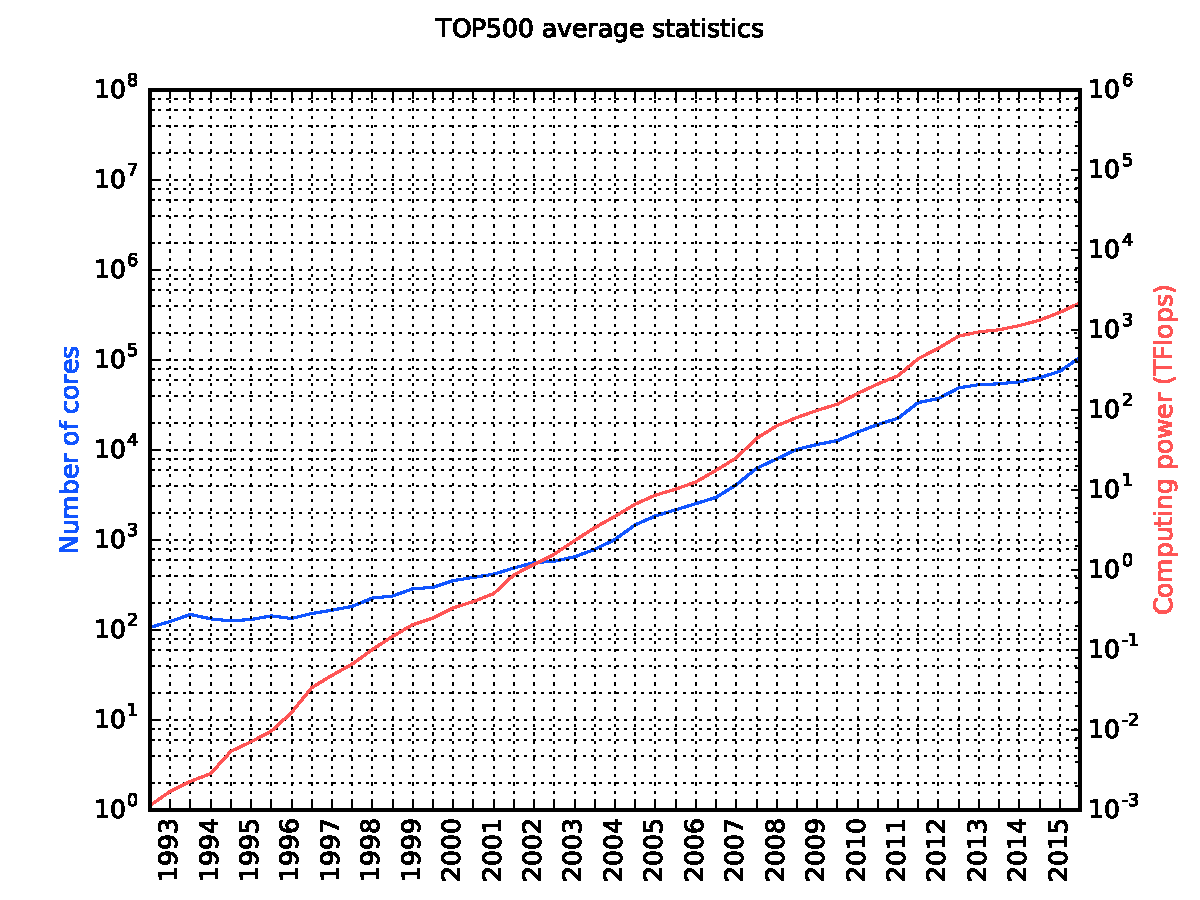
\includegraphics[scale=0.7]{img/cap1-top500-avg-comp}}
		\caption[TOP-500 supercomputers average performance]{Average number of cores and computing power of TOP-500
		supercomputers (TOP500.org data, retrieved 5 August 2016)}
		\label{fig:corestrend}
\end{figure}

\begin{figure}[t]
		\centerline 
{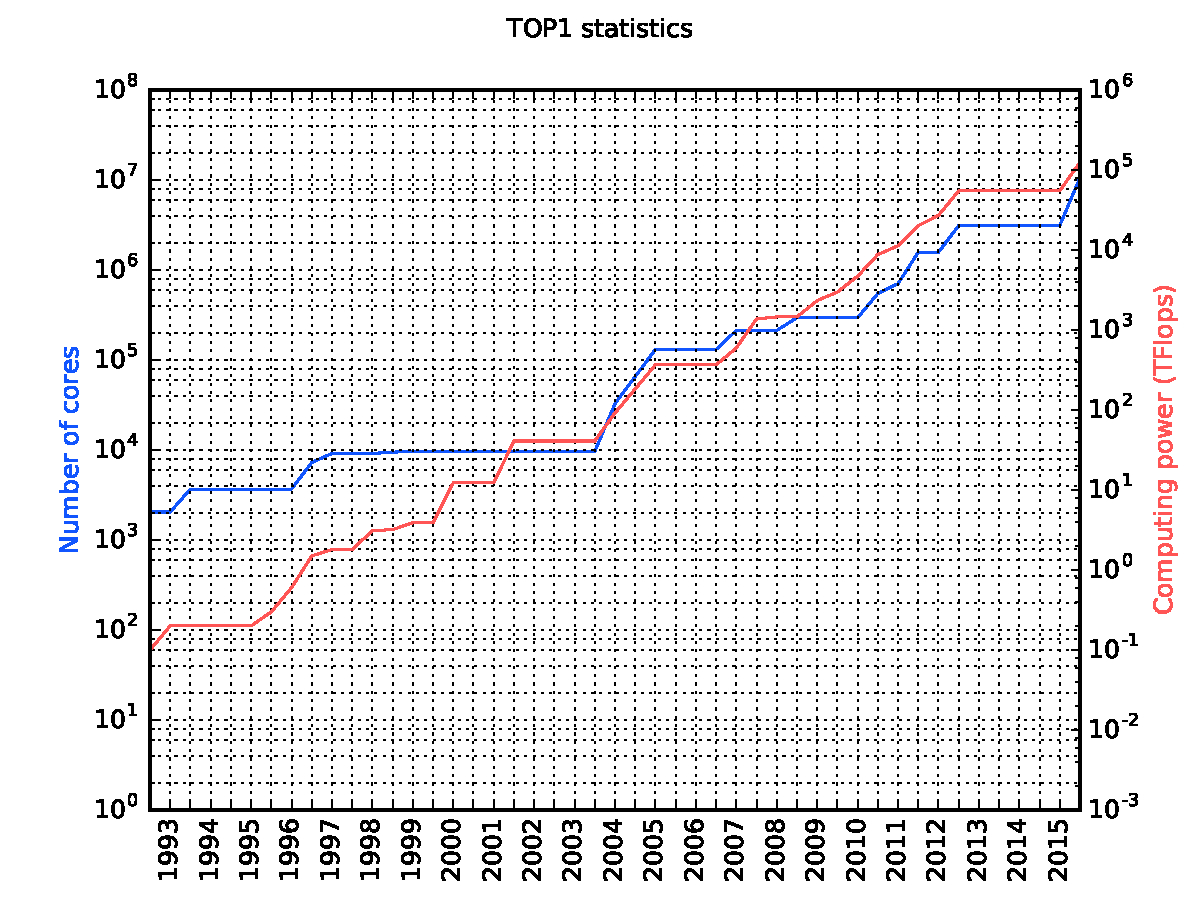
\includegraphics[scale=0.7]{img/cap1-top500-max-comp}}
		\caption[TOP-1 supercomputers performance]{Number of cores and computing power of the TOP-1
		supercomputer (TOP500.org data, retrieved 5 August 2016)}
		\label{fig:corestrend2}
\end{figure}


In last decades the rapid development of processing units maintained
acceptable levels of power consumption while increasing the performance
delivered. The computational units and computational power trends over
past two decades is shown in Figure \ref{fig:corestrend} and Figure
\ref{fig:corestrend2}.

Unfortunately, the miniaturization of semiconductors cannot go on forever,
thus the End of the \emph{Moore's Law} is one of the big concern. In fact,
the plateauing of voltage levels and the increasing of leaking current is
leading to a power wall \cite{Villa2014}.
The reduction of the performance increasing
trend, or even the reaching of a performance plateau, would significantly slow
down the scientific research \cite{snir2011exascale}. In 2014, the Department
of Energy of United States planned to achieve the too ambitious goal of
Exascale with 20 MW of power in 2018 \cite{USExascale}, but later the deadline
was extended.

\subsection{Exascale as a key goal to reach}
\textbf{Exascale computing} refers to systems having a minimum computing power
of more than 1 exaFLOPS, i.e. \( 10^{18} \) FLOPS.

Research towards Exascale is not limited to the computer science domain, but it
strongly affects all the areas of science and engineering. The increasing
complexity of mathematical models and the growing size of Big Data requires
a growing amount of computing resources.

The Exascale goal is in fact of great interest for a wide range of
applications. We can mention several examples, like the study of astrophysical phenomena, weather forecasting, product market simulations, the development of
new drugs, the analysis of health risks, etc.
\cite{Reed:2015:ECB:2797100.2699414}. For all these applications, Exascale
would enable the possibility of deploying more complex mathematical models,
capable of providing much more accurate and reliable results.


%%%%%%%%%%%%%%%%%%%%%%%%%%%%%%%%%%%%%%%%%%%%%%%%%%%%%%%%%%%%%%%%%%%%%%%%%%%%%%%
Vice versa, other non-computer scientists
are studying to find alternative technologies to the current one, in order to
mitigate the today issues. Several physicist are studying new types of
semiconductors, for instance the very promising research on silicon photonics
\cite{6476868}.

From the previous considerations we can state that HPC is still a very hot
topic of research and solving the related problematics is not just a matter
of computer science, but it will influence and it will be influenced by
the research activities in almost all fields.

%%%%%%%%%%%%%%%%%%%%%%%%%%%%%%%%%%%%%%%%%%%%%%%%%%%%%%%%%%%%%%%%%%%%%%%%%%%%%%%


\subsection{HPC systems architecture}
Since HPC systems require by definition high computational capabilities, the
computational resources are typically distributed across different high-end
machines (nodes). They are connected via a high speed networks, typically
10Gigabit Fiber Optics Ethernet or InfiniBand.

The storage is also provided through distribution solutions like
Storage Area Network (SAN) or Network Attached Storage (NAS).
Both solutions have to be designed for
HPC environment. In particular, the storage performance and capacity
should possibly scale linearly with the numbers of nodes and disks.

\begin{figure}[t]
		\centerline 
{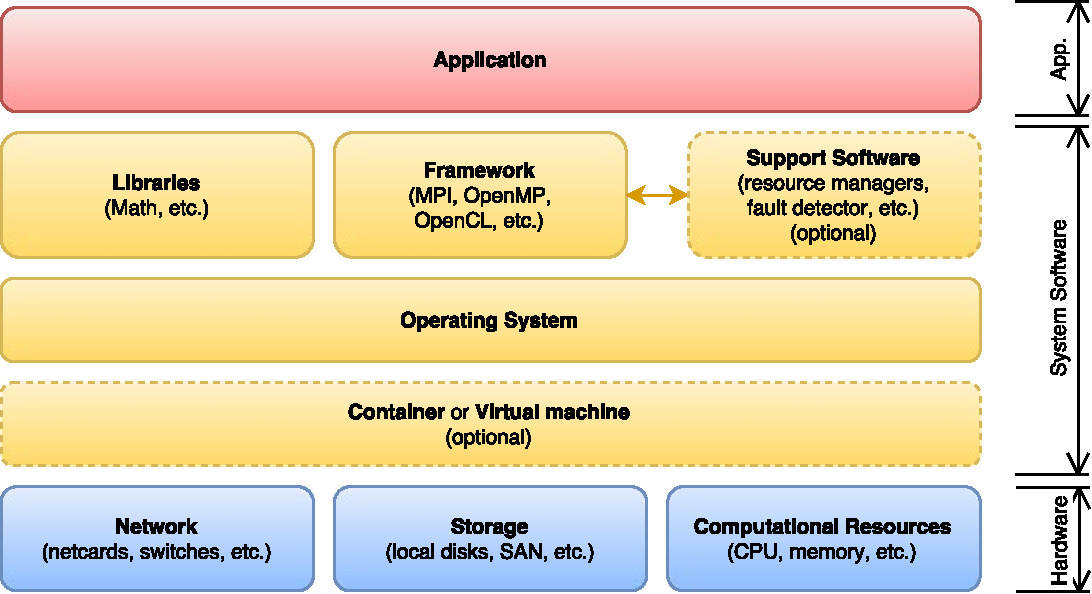
\includegraphics[scale=0.7]{img/cap1-generalarchitecture.pdf}}
		\caption[General architecture of a HPC node]{The general architecture of one node in a HPC system.}
		\label{fig:generalarchitecture}
\end{figure}

The general architecture of a single node in a HPC cluster is shown in
Figure \ref{fig:generalarchitecture}. End-user applications run over
a stack of software and, in particular, exploit the API provided
by a specific parallel programming framework like MPI or OpenMP. Since the
application computational requirements are far behind the performance
capabilities provided by a single CPU, the application must be designed in
order to run multiple threads or processes. Parallel frameworks
simplify the development of the applications, providing suitable API to
manage the execution of multiple tasks, the communication and the
synchronization among them.

Furthermore, the application may use other library providing specific
functionalities (e.g. math functions) or interact with
other software frameworks, like resource managers. The operating system as
usual provides to all of software the abstraction of the hardware (virtualized
or not).


\section{Dependability issues in HPC}
In HPC, dependability - a broad term including reliability, resilience,
fault tolerance, etc. - is another possible future wall in reaching
Exascale computing \cite{5871590}. To highlight the
size of the problem is sufficient to say that the Mean Time To Failure (MTTF)
for current HPC systems is way below 100 hours \cite{egwutuoha2013survey}.

The research community is therefore focusing its effort towards five key
directions \cite{cappello2014toward}:
\begin{enumerate}
\item statistical and technical characterization of hardware faults;
\item development of a standard fault interface from hardware to software;
\item improving fault prediction, containment, detection, notification and recovery;
\item the development of programming abstractions for resilience, especially fault-tolerant algorithms;
\item proposing fault-tolerant approaches both in hardware and software design.
\end{enumerate}

In this work, we focus on the item 4 proposing a tool that can be used
in HPC parallel applications in conjunction with a fault-detection mechanism to
support fault-tolerant executions on distributed systems.


\subsection{Fault-Tolerance requirements and techniques}
As already presented, one of the most important discussed theme in HPC is the
dependability concern. In particular, since the MTBF is very low compared
to the applications timespan, it is required fault-tolerance techniques
able to guarantee the termination of the application even if one or more faults
occur. In fact, some HPC applications take days or weeks to terminate and
after a fault a restart from the beginning is not acceptable. Therefore,
fault-tolerance is no longer a \emph{nice-to-have} feature, but it became a
\emph{mandatory} one in HPC systems.

To highlight the previous considerations, a simplification of
the Mean Time To Failure (MTTF) and Mean Time Between Failure calculus (MTBF)
is proposed, with the objective to provide a trivial qualitative analysis.
Assuming the system non repairable, thus \( \text{MTTF}=\text{MTBF} \),
let's consider a cluster of 1.000 CPUs Intel Xeon processor of E7 Family that has \(\text{MTTF}=100.000h\) (\textasciitilde 11y) \cite{E7Reliability}. The overall MTTF can be calculated as:

	\begin{equation}\label{eq:mttf1}
		\lambda_i = \frac{1}{\text{MTTF}_i}
	\end{equation}
	\begin{equation}\label{eq:mttf2}
		\lambda_{\text{overall}} = \sum{\lambda_i}^n
	\end{equation}
	\begin{equation}\label{eq:mttf3}
		\text{MTTF}_{\text{overall}} = \frac{1}{\lambda_{\text{overall}}}
	\end{equation}

Applying (\ref{eq:mttf1}), (\ref{eq:mttf2}), (\ref{eq:mttf3}) to our scenario:
\[  \text{MTTF}_{\text{overall}} = \frac{1}{ 1.000 \cdot \frac{1}{100.000} }
 = 100h \]

The overall MTTF was drastically reduced from 11 years to just few days.
Please also note that modern supercomputers have more than 30.000 physical
CPUs, leading to MTTF to be less than 4 hours. It is clear that most of the
HPC applications, that requires more than few hours to conclude, need a
sort of abstract of a fault-free system, in order to execute ideally without
being affected by hardware faults. Several approaches have been proposed in
literature and industry. The state of the art of this techniques will be
discussed in the next chapter.

\subsection{Failures taxonomy and sources}
Following the classification provided by \emph{Snir et al.}
\cite{snir2014addressing}, the HPC failures may be grouped in three
categories: \emph{detected and corrected by the hardware} (DCE), \emph{detected
but not corrected by the hardware} (DUE) and \emph{non-detected silent errors}
(SE).
We do not consider DCE, since they are transparent to the software; for
instance, the ECC memory correction is an example of DCE and it is usually
performed transparently to the software. We neither deal with SE: the
correctness of the result has to be checked by the application since the
framework has no tool to infer it.

In the example about the calculation of MTTF, the CPU fault rate was
considered. However, other components like memory may be the source of
the failure, further deteriorating the reliability. Regarding \textbf{hardware faults}, they can be divided -
following the \emph{Snir et al.} classification - in \emph{compute soft},
\emph{compute hard}, \emph{network}, and \emph{I/O} errors. Vice versa,
\textbf{software faults} can be classified in: \emph{pure software}, 
\emph{hardware propagating up}, and \emph{software propagating down} errors. 
This taxonomy is better presented in the subsequent 
Table \ref{tab:faulttaxonomy}.


\begin{table}[ht!b]
\centering
\begin{tabular}{ c|c|c}

\multirow{4}{*}{\parbox{2.5cm}{\vspace{2cm}Hardware faults}} 
 & \centering Compute soft errors & \parbox{6cm}{\vspace{.5\baselineskip}
 Errors caused by transient
 faults in electronics,  e.g. memory corruptions caused by an electromagnetic
 interference
 \vspace{.5\baselineskip}}
 \\ \cline{2-3}
 & \centering Compute hard errors & \parbox{6cm}{\vspace{.5\baselineskip}
 Permanent fault of a
 computational component (CPU, RAM, etc.) due to a physical problem, e.g.
 electromigration.
 \vspace{.5\baselineskip}}
 \\ \cline{2-3}
 & \centering Network errors & \parbox{6cm}{\vspace{.5\baselineskip}
 Total or partial loss of network
 connectivity, often caused by external component w.r.t. machine, e.g.
 network apparatus failures.
 \vspace{.5\baselineskip}}
 \\ \cline{2-3}
 & \centering I/O errors & \parbox{6cm}{\vspace{.5\baselineskip} Transient or
 systematic errors during
 the reading or writing to disks or other storage
 \vspace{.5\baselineskip}} \\ \hline
\multirow{3}{*}{\parbox{2.5cm}{\vspace{1.3cm}Software faults}} 
 & \centering Pure software errors & \parbox{6cm}{\vspace{.5\baselineskip}
 The category containing the
 classical programming issues: correctness errors, concurrency errors, etc.
 \vspace{.5\baselineskip}}
 \\ \cline{2-3}
 & \centering HW propagating to SW & \parbox{6cm}{\vspace{.5\baselineskip}
 A bug in the hardware that
 propagates up to the software, typical an unmanaged DUE.
 \vspace{.5\baselineskip}}\\ \cline{2-3}
 & \centering SW propagating to HW & \parbox{6cm}{\vspace{.5\baselineskip}
 A bug in the software that
 damages the hardware; it is typical of firmware in embedded appliances.
 \vspace{.5\baselineskip}}\\ 

\end{tabular}

\caption[The fault taxonomy in a HPC environments]{The fault taxonomy in a HPC system according to
\emph{Snir et al.} classification.}
\label{tab:faulttaxonomy}

\end{table}


The number of possible faults that may lead to a failure in the system
and/or in the running HPC applications explains why the thematic of fault
tolerance is today not only bound to the embedded world, but it has a
fundamental importance also for HPC environments.

\subsection{Checkpoint/Restart}
In response to these faults, most of long-run jobs require a
\textbf{Checkpoint/Restart (C/R)} mechanism. The C/R paradigm
consists in performing periodic \emph{checkpoints}, i.e. save the
status of the system on non-volatile memory, in order to \emph{restart} the job if a fault occurs. The restart
is triggered after the fault is detected and corrected.

Provided the images are saved in a persistent storage
\footnote{In this context \emph{persistent storage} is intended as fault-free
non-volatile memory.}, this
technique guarantees the ability to recover from any type of fault.
However, the cost of checkpoint is extremely high and it has to be executed
periodically. The overhead can easily reach 50\% of the total execution time,
reducing considerably the impact on the efficiency of the system
\cite{fiala2012detection}.

\subsection{Performance variation and degradation}
Performance variation and degradation are increasing problems in
semiconductors. The component aging has an important effect in
these two problematics.

In HPC, not only faults have to be taken in account: the performance
degradation and fluctuation affect also the overall performance of the
jobs. Then, it makes important to preserve an acceptable level of aging
of all components, through periodical maintenances. Unfortunately,
most of operations on machines require to shutdown it; in this direction,
migration allows a system administrator to request the freeing of a machine
without  the necessity to wait the completion of current tasks or freeze
entirely the job via C/R.

\section{Resource management in HPC}
The resources management in supercomputers is a prominent challenge. 
Resource allocation in HPC is a problem studied since 1980s, trying to
find a model to allocate jobs in optimal distribution across supercomputers.
Albeit the question is old, the increasing of resources spread over several
nodes and the diversity of the
software require specific policies to schedule and allocate jobs over the
cluster. In this regard, we may choose between applying static or dynamic
policies. Static policies are in most cases suboptimal or totally inadequate
to manage parallel workloads. While dynamic policies allows us to adapt
resource allocation decisions to the current workloads characteristics and
system status. Moreover, heterogeneous computing
is considered by AMD one of the essential capabilities to reach
Exascale computing \cite{7155462}.

The goal of this policies may be vary, for instance obtain the maximum
performance for certain category of applications or reduce the
resource underutilization to minimum, in order to maintain an efficient system.
Different applications may have different priorities or they have to generate
results (e.g. predictions) within a given mandatory rate. In this case, it's
more important to satisfy the strongest
requirement than to have the maximum efficiency.

Most of the large clusters are utilized not only for HPC, but also for Cloud
Computing. This mixed environment requires to manage different types of
workloads: resource-intensive long-run for HPC applications and a resource
flexible adjustment for Cloud. Resource management techniques capable of
dealing with mixed workload are consequently required \cite{chen2013dynamic} for large computing centers.

In 2016 \emph{Cela et al.} provide an overview \cite{cela2016fostering} of
energy-related issues in new exascale HPC applications. Resource management
at MPI level is considered essential in order to achieve high scalability.
One of the main topics proposed for future research is precisely the migration
of MPI processes, that is the main topic of this work. Migration opens up a 
wide range of possibilities. For instance the resource manager can adapt the
computing resource assignment to time varying application performance
requirements. Moreover, the application load can be balanced among the system
nodes, in order to level down the power consumption and the temperature peaks.

This thesis presents a novel migration technique in MPI and its integration and
exploitation in Barbeque RunTime Resource Manager, a resource manager part of the BOSP open source project.

\section{Message Passing Interface}
The \textbf{Message-Passing Interface} standard (abbreviated in MPI) is
the \emph{de-facto} standard for parallel computing across different
nodes. 
The MPI Forum - composed by both academic and industrial
people - released the first version of this standard in 1994 and the last
version (3.1) was released in 2015\cite{mpistd}. 

The MPI standard describes the syntax and the semantics of function calls in
the Application Program Interface (API) provided by a MPI library to the user
software. This API allows the communication, the management and the
coordination between processes of a parallel application. MPI is mainly
used for distributed computing, despite in theory it can be used for the
execution on local machine only. In the latter case, \emph{OpenMP} is usually
preferred, since it is optimized specifically for single node executions.
To reach better performance, most applications are implemented combining
the usage of MPI and OpenMP together.

The MPI standard is written through
a language-independent specification, in order to be implemented in any
programming languages. The most common languages are C, C++ and Fortran.

\begin{figure}[t]
		\centerline 
{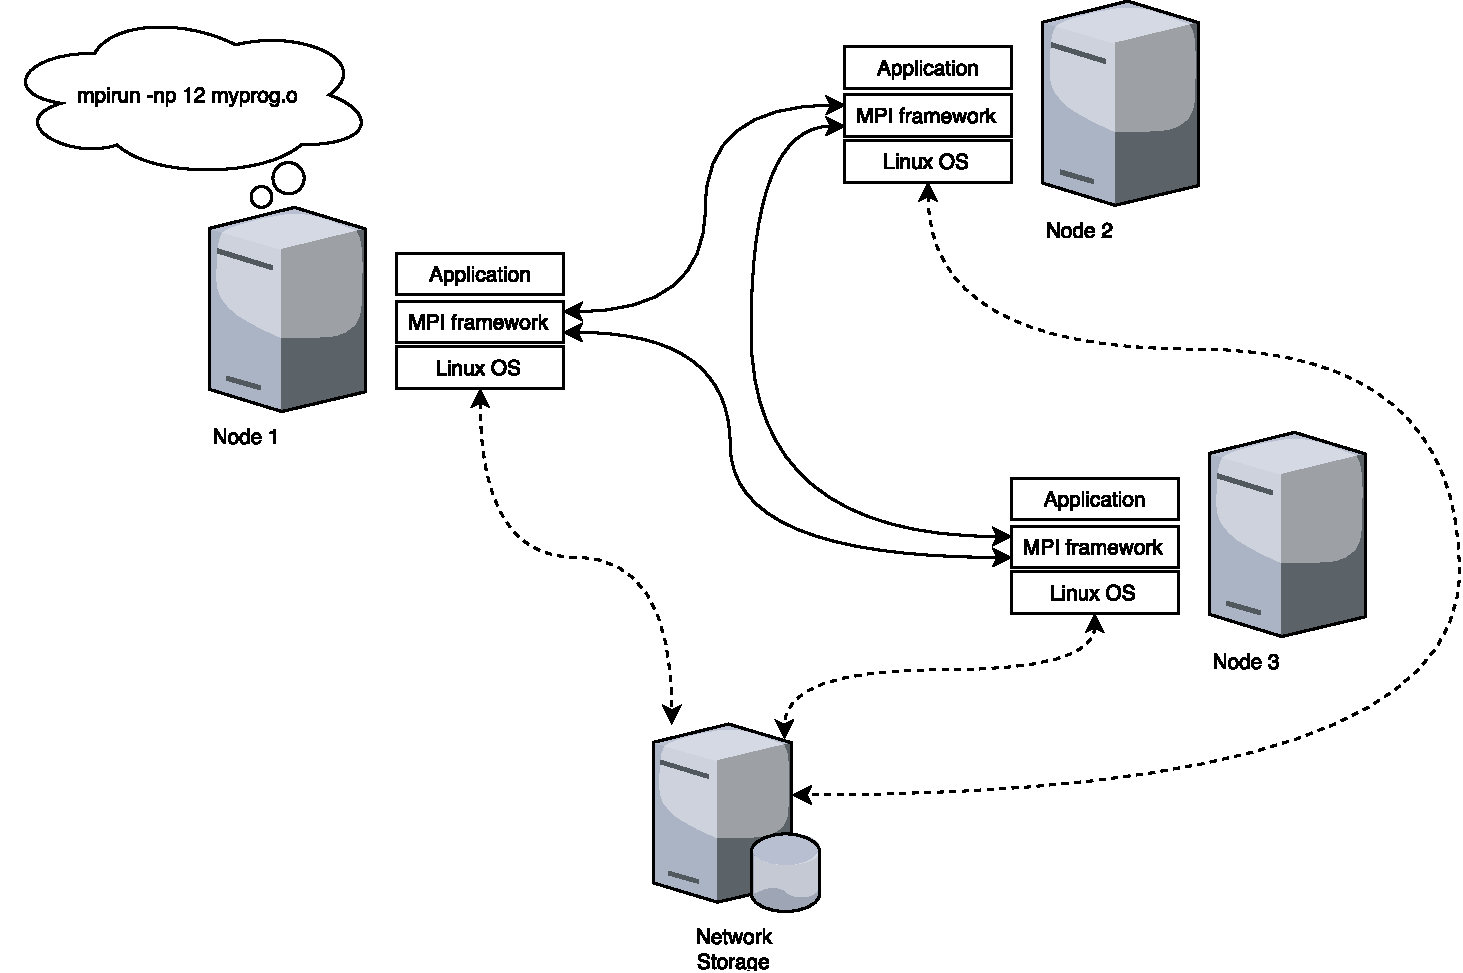
\includegraphics[scale=0.5]{img/cap1-mpiarchitecture.pdf}}
		\caption[MPI systems typical setup] {A typical configuration of MPI systems: the user launches the
		\texttt{mpirun} command on Node 1 that distributes the computation
		also over the Node 2 and Node 3. All nodes have access to a common 
		network storage to get the program and the data.}
		\label{fig:cap1-mpiarchitecture}
\end{figure}


\subsection{MPI Application Execution Flow}
A MPI typical MPI execution is presented in Figure 
\ref{fig:cap1-mpiarchitecture}. The user launches the job via the
\texttt{mpirun} command, then the MPI framework spawns the processes
in the other available machines (how this is performed is implementation
dependent).

The application must be linked with the static or dynamic library of MPI,
that provides \texttt{MPI\_*} function calls. Usually every program starts
with \texttt{MPI\_Init} and ends with \texttt{MPI\_Finalize}. Both functions
are implementation-dependent, but in general \emph{MPI\_Init} performs some
setup required before any other MPI routines and the
\texttt{MPI\_Finalize} coordinates the execution conclusion freeing the
allocated resources.

The communication between processes is divided in two categories:
\emph{point-to-point} (direct communication between two processes) and
\emph{collective}
(communication one-to-many or many-to-many). The latter is performed through
the coordination of the various MPI frameworks on all nodes. A typical example
of collective feature is the \emph{barrier}: every program should synchronize
at the same point before continuing.

Having a common set of functions allows to perform easily and equivalently
benchmarks of the same application on different MPI frameworks or to port
the program on another framework without refactoring the code.

\subsection{MPI implementations}

Today, several implementations of MPI are available, among which we cite
the two most commonly used: MPICH\cite{karonis2003mpich} and Open
MPI\cite{gabriel2004open}. They are both open source and have reached a good
level of stability even with a considerable number of features, thanks to the
very active communities and the large funding of big companies and
universities.

The history of MPICH can be split in two part: MPICH-1 and MPICH-2. The
development of the latter (at a later time called simply MPICH) starts in
2001 to add the feature of MPI version 2 and subsequently version 3 to MPICH-1.

Open MPI represents the union of three
previous implementations: LA-MPI, FT-MPI and LAM/MPI. The third 
was extensively used in research literature. All of which ceased their
development shortly after the begin of Open MPI project in 2003.

The two implementation mainly differs in the purpose of application: MPICH is
a very stable basis and standard reference for the development of special
purpose needs. Open MPI targets more general cases and it already offers
several pre-implemented features, e.g. different types of network
communication channels and topology.

Since our framework is supposed to be a general tool that tries to address
the issues of the most of HPC applications, we selected the Open MPI
implementation to develop the feature presented in next sections. Furthermore,
the extreme high modularity of Open MPI internal code was a big advantage in
the development of \texttt{mig} framework\footnote{Note that the keyword
`framework` may generate misunderstanding: as explained in Chapter
\ref{cap:design}, the \texttt{mig} framework is a module of Open MPI, not a new
MPI framework}.


\section{Migration of MPI processes}
This thesis presents a technique implemented in Open MPI able to allow the
migration of MPI processes among different nodes of the cluster. Moving a
process across different machines is not a straightforward task and
it constitutes a specific research topic. This work exploits existing
process migration tools applying them to Open MPI for HPC applications.

Migration of processes can be exploited to solve or mitigate some of the
previous presented issues. Obviously, the migration is not for free and
introduces an overhead that must
be taken in account, while being triggered by an appropriate software, for
instance by a fault detector or a resource manager.

Migration is particularly interesting for resource management: current runtime
resource managers in HPC are limited to assign resources during the application
startup, therefore they are not usually able to reschedule the application over
different nodes. Migration adds the capability of rescheduling to resource
managers, that they have to take in account the significant overhead of
moving processes between two nodes.

In large clusters the topology and consequently the location of the processes
of the same job significantly impacts on overall performance; even if
all nodes are in the same network, the distant of two machines noticeable
affects the network performance. If the topology of the cluster changes -
despite the application is not involved - a rescheduling may be convenient
to reach better performance. Since C/R is too expensive in terms of time and
required resources, this scenario can be an interesting exploitation of
migration techniques.

Regarding fault tolerance, the migration may in fact lead to a the reduction
of the number of C/R required:
an appropriate pre-fault detection system would trigger the migration if an
imminent fault is detected, avoiding the long restart required if the fault
happens.

Certainly, a sudden unexpected undetectable fault is not manageable with
a migration technique. This is why C/R mechanisms cannot be fully replaced.
Instead, the frequency of the checkpoints can be effectively reduced,
provided an appropriate fault probability analysis.

The software architecture considered for this work does not provide a fault
detector, but assume the presence of an external one that signals the resource
manager in case of imminent fault. Subsequently, the resource manager and the
MPI framework will trigger the migration. With this setup, the resource
manager is the only interlocutor with the MPI framework and it can allocate
and possibly reallocate resources over available nodes.

\section{Thesis structure and objectives}
The main topic of this thesis is a novel approach to process migration
implemented in Open MPI. This technique was also presented at the EuroMPI 2016
conference\cite{myEuroMPI}. In addition, the exploitation of this technique
with the \textbf{Barbeque Run-Time Resource Manager} (from now simply
\emph{BarbequeRTRM}) is presented in conjunction with a basic centralized
resource management policy for distributed systems.

In Chapter \ref{cap:state-of-the-art} the State of the art related to
migration and C/R techniques is discussed and the novelty of the
proposed method is highlighted. The Open MPI and CRIU frameworks are
described in Chapter \ref{cap:ompicriu}. Subsequently in Chapter
\ref{cap:design} and \ref{cap:integration} the design, the implementation and the integration with
\emph{BarbequeRTRM} are explained, detailing and arguing all design choices.
The testing results are discussed in Chapter \ref{cap:evaluation}, focusing on
the introduced overheads. Eventually, in Chapter \ref{cap:discussion} future
research directions and developments are proposed. It is also the thesis end containing the conclusions.   
 
\chapter{State of the Art}
\label{cap:state-of-the-art}

\section{Self-Adaptive Software Systems}
\label{sec:sas}
In modern-day applications, software complexity has extremely increased thanks to the spread of highly available and faster wireless connection such as in the Internet of Things (IoT) ambit. Since software is often deployed in dynamic contexts, where requirements, environment assumptions and usage profiles vary continuously, software complexity increased over time to the point where it is often composed by a number of sub-components and/or sub-services that work together in order to offer a service to the users. This is the case of service-oriented applications -- also called Service Based Systems (SBS) -- that are composed by multiple \emph{services} and \emph{components}. In these systems, services offered by third-party providers are dynamically composed into workflows to deliver complex functionalities, so SBSs rely on self adaptation to cope with the uncertainties associated with third-party services as the loose coupling of services makes a reconfiguration feasible. Without adaptation, the application is prone to degraded performance  because of faulty components, messages lost between services or delays due to an increasing number of users.

During the past decade a lot of research has been made in this scope but the engineering of adaptive systems remains an incredible challenge\cite{soft-eng-for-sas-2}. In order to solve the problem, \textbf{Self-Adapting Software Systems (SASS)} are born. These are flexible systems that can adapt themselves to their contextual needs and can do so with the highest performance and availability. General discussion concerning the issue and the state of the art in the design and implementation have been presented\cite{soft-eng-for-sas-2}\cite{survey-aut-comp}\cite{self-adap-soft}\cite{soft-eng-for-sas-1}\cite{soft-eng-for-sas-3}\cite{arch-based-appr-to-sas}\cite{sas-quant-ver}.

These kind of systems have some fundamental properties called auto-managing that are:
\begin{itemize}
	\item Auto-configuration
	\item Auto-recovery in case of failure
	\item Auto-optimization
	\item Auto-protection
\end{itemize}
All these properties can be grouped in two more abstract concepts which are self-awareness and context-awareness.

\textbf{Self-Awareness} is the ability of the system to be able to monitor itself in terms of available resources and behavior.

\textbf{Context-Awareness} is the ability of the system to understand the environment where it is working, using the information provided by its components, and adapt itself to all the changes that can occur during its normal operational status.
To better understand how a SASS works we need to answer some simple questions:
\begin{itemize}
	\item Who is adapting?
	\item What adaptation is required?
	\item When is it necessary to adapt?
	\item Where is it needed to change something?
	\item Why is it needed an adaptation?
	\item How do we achieve this goal?
\end{itemize}

During the past years have been developed some dimensions that help to answer all this simple questions: \emph{Time}, \emph{Reason}, \emph{Level}, \emph{Technique} and \emph{Adaptation Control} shown in Figure \ref{fig:dimensions}.
\begin{figure}[ht]
	\centerline
	{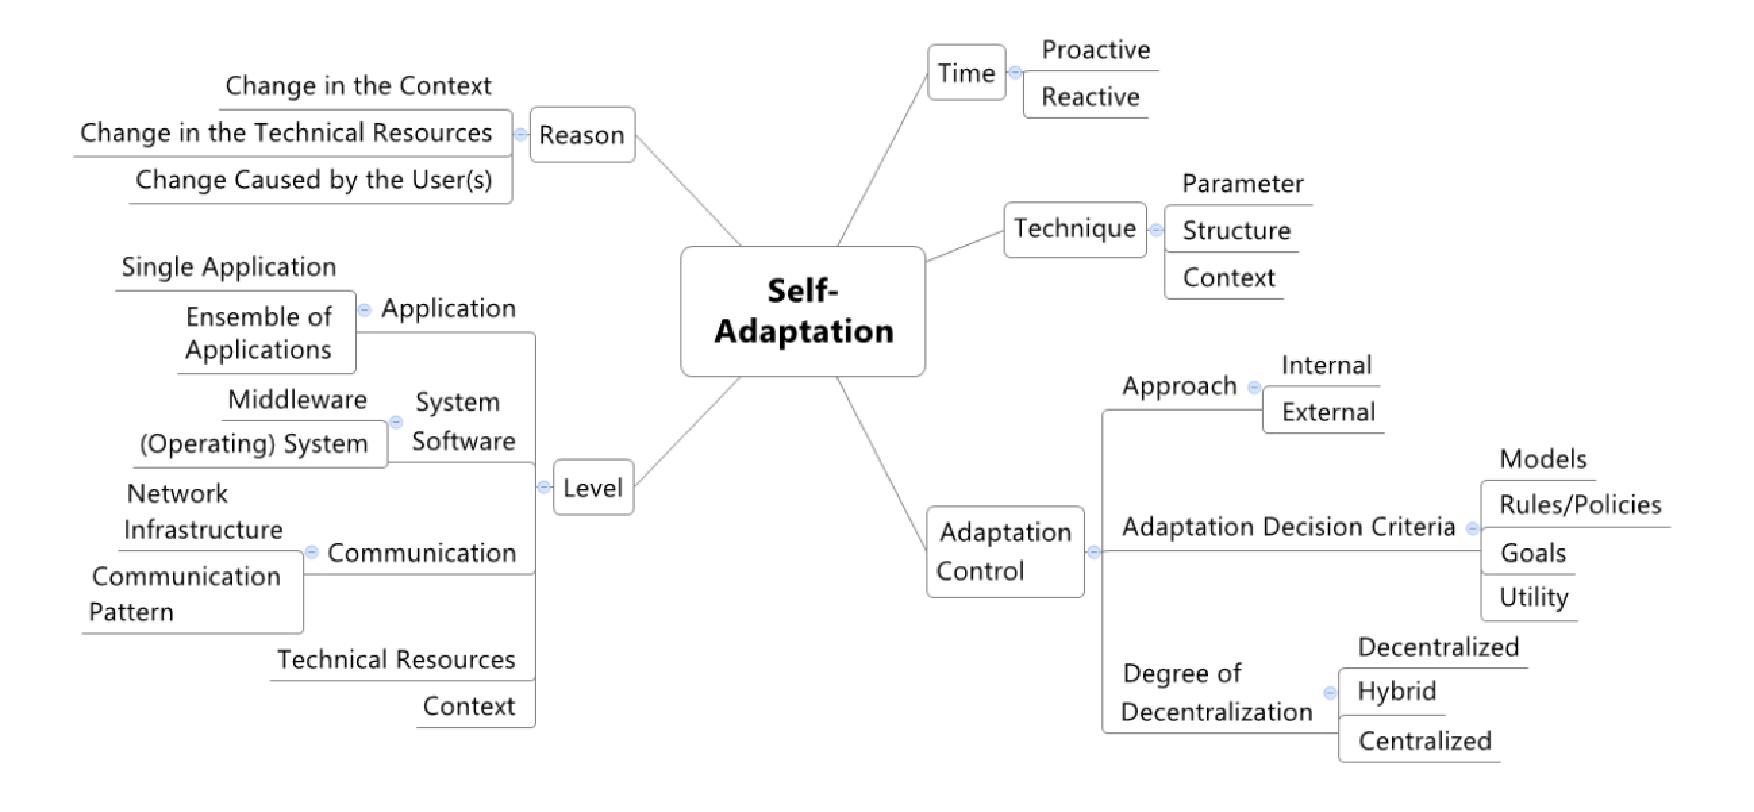
\includegraphics[scale=0.50]{img/dimensions.png}}
	\caption[The Dimensions]{The Dimensions to analyze adaptation.\cite{eng-appr-sas}}
	\label{fig:dimensions}
\end{figure}

\textbf{Who is adapting?} As the name suggests, it's the system itself that changes something in order to preserve some given constraint.

\textbf{What adaptation is required?} The \emph{Technique} dimension is the one that answers this question in fact the software engineer can change either the parameters or the system can be considered as a set of components. The former case allows to fine tuning the system at the expense of an higher complexity, the latter is called composite vision and permits the systems to cooperate exchanging algorithms and much more important, reusing components which improve performance because failed or defected components can be replaced.

\textbf{When it is necessary to adapt?} The \emph{Time} dimension is crucial in this situation. There are three typical approaches: the reactive one is the more traditional one which states that an adaptation is needed only after a causative event. The other two approaches are more interesting and they are predictive and proactive. The former studies the system before any event and calculate the need of an adaptation, the latter applies and adaptation despite an event and improves the performance. From the user perspective the proactive approach is the best because it doesn't interrupt the operation of the system in any load but it is the more complicated to implement. Monitoring continuously the system is a costly task to do, on the other side an adaptive monitoring is simple that analyze only specific aspect and/or resources and intervenes only if needed.

\textbf{Where it is needed to change something?} In general a SASS is composed by two main part: the the Adaptability Logic (AL) and the Managed Resource (MR). The former in general doesn't change, the latter is composed at the base of the hardware and of the software such as the operating system or, in case of distributed systems, the middleware that control the hardware; at a higher level of the application. These are the parts that require adaptation. To answer this question is needed to decide at which level the operation has to be applied without neglecting the relationship between the MR and the AL which is composed by the network that connects them and/or the view of the communication patterns. Thus \emph{Level} is the considered dimension.

\textbf{Why it is needed an adaptation?} In this case, \emph{Reason} is the right dimension. There can be one or more reason because a system needs adaptation such as a change in the available resources, a change in the environment or a change in the user base of the system.

\textbf{How do we achieve this goal?} The answer to this question is more complicated than the others because it needs a new topic called \emph{Adaptation Control}.

\subsection{Adaptation Control}
In the literature can be found 2 approaches: the \emph{internal approach} that intertwine the adaptation logic with the system resources, which has problems with the maintainability and scalability of the system, and the \emph{external approach} that splits the system into adaptation logic and managed resources, which increases maintainability and scalability through modularization.

The control unit needs a metric in order to decide how to adapt and in literature different metrics are present: models, rules and policies, goal or utility functions \cite{autonomic-computing}.

Another aspect of the adaptation logic is the degree of decentralization. If we have a system with limited resources then a centralized adaptation logic has to be preferred but with greater systems a decentralized AL can improve performance and  every sub-system can communicate with another with different patterns of communication. Of course hybrid technique can be made mixing the previous approaches.

\subsubsection{Adaptation Logic Issues}
As said before a SASS is composed of managed resources and the adaptation logic; it can be represented by the tuple \texttt{SASS = (AL, MR)}. \emph{AL = $a_1$, \dots, $a_n$}, with $a_i$ representing a logic element,  monitors the environment (M), analyzes the data for change (A), plans adaptation (P) and control the execution of the adaptation (E): these are known as \emph{MAPE cycle} or \emph{MAPE functionality}\cite{vision-aut-comp}. \emph{MR = $mr_1$, \dots, $mr_n$}, with $mr_i$ representing a resource, is the set of resources such as hardware with software, smart-phones, robotics or unmanned vehicles. Figure \ref{fig:sass} shows a SASS where the dashed line represent the system border.
\begin{figure}[ht]
	\centerline
	{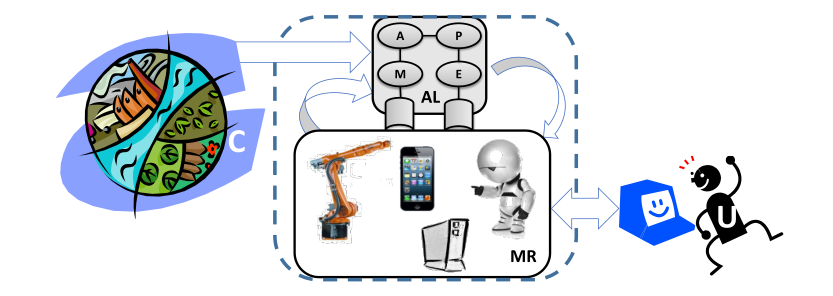
\includegraphics[scale=0.55]{img/managed-resources.png}}
	\caption[A SASS]{A SASS (AL = Adaptation Logic, MR = Managed Resources, U = User(s), C = Context, M,A,P,E = MAPE functionality).\cite{eng-appr-sas}}
	\label{fig:sass}
\end{figure}
The dimension can therefore be mapped to the MAPE functionalities as shown in table \ref{tab:mape}.
\begin{table}[ht!b]
	\centering
	\begin{tabular}{|l||p{2.4cm}|p{2.4cm}|p{2.4cm}|p{2.4cm}|}
		\hline 
		& \textbf{Time} & \textbf{Reason} & \textbf{Level} & \textbf{Technique} \\ 
		\hline 
		\textbf{Monitoring} & Continuos & What to monitor & Identification of the levels & --- \\ 
		\hline 
		\textbf{Analyzing} & Algorithms depend on reactive or proactive dimension & Where to analyze & --- & --- \\ 
		\hline 
		\textbf{Planning} & --- & What should be influenced by planning & Adaptation plans address these levels & Plans for performing the techniques \\ 
		\hline 
		\textbf{Executing} & --- & --- & Execution of the change on the levels & Execution of the change on the levels \\ 
		\hline 
	
	\end{tabular} 
\caption[MAPE and Dimensions]{Relation of the MAPE Activities and the Dimensions}
\label{tab:mape}
\end{table}

\section{The SOLAR Framework}
\label{sec:solar-framework}
Working on the adaptability of a system can impact other quality attributes such as performance, reliability or maintainability and in the worst case improving adaptability can decrease part, if not all, of these attributes as stated in \cite{bass2003software}: \emph{quality attributes can never be achieved in isolation, the achievement of any one will have an effect, sometimes positive and sometimes negative, on the achievement of others}.

Find a balance between these quality attributes is often a challenging task because sometimes they're conflicting each other, e.g. lower cost and higher availability, so find an adaptability value that can meet all the requisites is, as a consequence, a challenging task too.

The SOLAR (SOftware quaLities and Adaptability Relationships) framework \cite{solar} helps the software architect to select the best set of components in order to fulfill the requirements trying to achieve a minimum level for some quality attribute such as availability and/or cost. This tool helps the software architect to build a suitable architecture for his needs but is not a \emph{"solution for every situation"}.

\subsection{The SOLAR Metrics}
\label{subsec:solar-metrics}
All the metrics in SOLAR are greatly inspired by \cite{po-metrics} and are all defined at an architecture level and static perspective. 

To define them, the software architecture relies on a component-and-connector view (C\&C view). In this C\&C view \emph{components} are principal computational elements present at runtime. The representation used in Figure \ref{fig:comp-example} uses the UML diagram and shows some components and their respective connections.

\begin{figure}[ht]
	\centerline
	{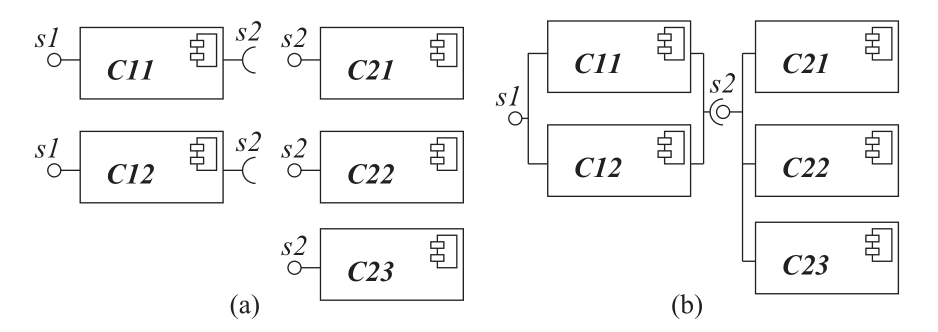
\includegraphics[scale=0.55]{img/solar-comp-example.png}}
	\caption[SOLAR Components example]{(a) A set of components and their interfaces and (b) the C\&C view of the components in (a)\cite{solar}.}
	\label{fig:comp-example}
\end{figure}

Components have interfaces attached to ports. \emph{Connectors} are pathways of interaction between components and also have interfaces or roles. In Figure \ref{fig:solar-arch-example} it is shown an example of an architecture, the used components are highlighted in gray; this example will be used to explain the metrics later in this chapter.

\begin{figure}[ht]
	\centerline
	{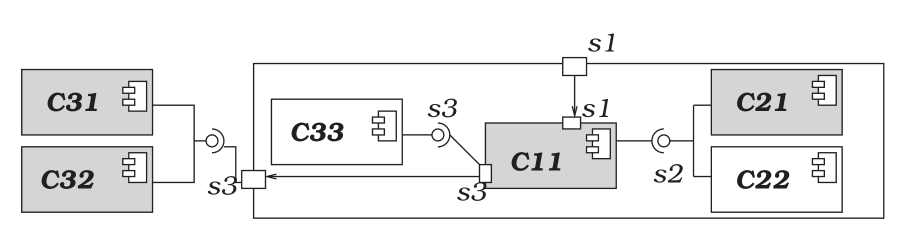
\includegraphics[scale=0.55]{img/solar-arch-example.png}}
	\caption[SOLAR example architecure]{C\&C view: discovered components and used components (in gray).\cite{solar}}
	\label{fig:solar-arch-example}
\end{figure}

In the architecture of Figure \ref{fig:solar-arch-example}:
\begin{itemize}
	\item the service S1 is provided by component C11 that is unique and must be in use. S1 is the provided service of this architecture.
	\item component C11 requires S2 and S3 services.
	\item service S2 is provided by C21 and C22 where only C21 is in use.
	\item service S3 is provided by C31, C32 and C33 but only C31 and C32 are in use.
\end{itemize}

\subsubsection{Absolute adaptability of a service (AAS)}
This metric measures the number of used components for providing a given service.
\[ AAS \in \mathbb{N}^n |AAS_i = |UC_i|\]
Quantifies how much adaptable a service is by counting the different alternatives to execute the service (1 no adaptable, $>$1 adaptable), where the service adaptability grows according to the number of components able to provide it. 

\noindent Referring to the example in Figure \ref{fig:solar-arch-example}, we observe that $AAS = [1, 1, 2]$.

\subsubsection{Relative adaptability of a service (RAS)}
This metric measures the number of used components that provide a given service with respect to the number of components actually offering such service.
\[ RAS \in \mathbb{Q}^n | RAS_i = \frac{|UC_i|}{|C_i|} \]
It describes how each service stresses its adaptability choices and it informs how much more adaptable the service could be. RAS vector values near to one mean that the service is using almost all the adaptability potentially reachable. 

\noindent Referring to the example in Figure \ref{fig:solar-arch-example}, we observe that $RAS = [1, 0.5, 0.6]$.

\subsubsection{Mean of absolute adaptability of services (MAAS)}
This metric measures the mean number of used components per service.
\[ MAAS \in \mathbb{Q} | MAAS = \frac{\sum_{i=1}^{n} AAS_i}{n}  \]
It offers insights into the mean size and effort needed to manage each service.

\noindent Referring to the example in Figure \ref{fig:solar-arch-example}, $MAAS = 4/3 = 1.3$. 

Architectures with more adaptable services have higher values of MAAS. Besides, a $MAAS > 1$ means that the architecture includes adaptable services (at least one of the components $AAS_i > 1$). For $MAAS \le 1$, there may be adaptable services or not (AAS should be checked in this case).

\subsubsection{Mean of relative adaptability of services (MRAS)}
This metric represents the mean of RAS.
\[ MRAS \in \mathbb{Q} | MRAS = \frac{\sum_{i=1}^{n}RAS_i}{n}\]
It informs about the mean utilization of the potential components for each service. Values of this metric range between zero and one.

\noindent Referring to the example, $MRAS = (1 + 0.5 + 0.6)/3 = 0.72$.

The higher the MRAS of an architecture, the more adaptable its services are, on average. The maximum value of this metric is obtained when $RAS_i = 1 \;\;\forall i \in [1, \dots, n]$, which is in turn obtained when all services are as much adaptable as possible because they use all the available components. Therefore, a value close to one for MRAS means that, on average, services are as much adaptable as possible. A value close to zero means that: 
\begin{enumerate}
	\item[\textbf{a)}] services can be much more adaptable (adding components not yet used)
	\item[\textbf{b)}] different architecture alternatives with the same quantity of adaptability can be created
\end{enumerate}

\subsubsection{Level of system adaptability (LSA)}
This metric measures the number of components used to make up the system with respect to the number of components that the most adaptable architecture would use.
\[ LSA \in \mathbb{Q}{0..1} | LSA = \frac{\sum_{i=1}^{n}AAS_i}{\sum_{i=1}^{n}|C_i|} \]
The value of this metric ranges between zero and one. For LSA, a value of one means that the system is using all existing components for each service, i.e., $AAS_i = |C_i | \forall i \in {1,\dots, n}$, and then its adaptability is already to the maximum. A value close to one means that the market offers few choices to increase the system architectural adaptability. When a new component is bounded to the architecture, LSA increases in a constant value ($1/\sum{{i=1}^{n}|C_i}$) irrespective of the number of components already considered for the same service.

\noindent Referring to the example in Figure \ref{fig:solar-arch-example}, $LSA = 4/(1 + 2 + 3) = 0.6$.

Table \ref{tab:solar-metrics-summary} summarizes the five metrics and their values for the example in Figure \ref{fig:solar-arch-example}.

\begin{table}[ht!b]
	\centering
	\begin{tabular}{|l|l|l|l|}
		\hline 
		Name & Range & Value & Example in Fig. \ref{fig:solar-arch-example} \\ 
		\hline 
		AAS & $\mathbb{N}^n$ & ${|UC_i|}$ & $[1,1,2]$ \\

		RAS & $\mathbb{Q}^n \in {0,\dots,1}$ & ${\frac{|UC_i|}{|C_i|}}$ & $[1,0.5,0.6]$ \\ 

		MAAS & $\mathbb{Q}_+$ & $\frac{\sum_{i=1}^{n}AAS_i}{n}$ & $1.3$ \\ 

		MRAS & $\mathbb{Q}^n \in {0,\dots,1}$ & $\frac{\sum_{i=1}^{n}RAS_i}{n}$ & $0.72$ \\ 
		
		LSA & $\mathbb{Q}^n \in {0,\dots,1}$ & $\frac{\sum_{i=1}^{n}AAS_i}{\sum_{i=1}^{n}|C_i|}$ & $0.6$ \\
		\hline 
		
	\end{tabular} 
	\caption[SOLAR Metrics]{Summary of the metrics.\cite{solar}}
	\label{tab:solar-metrics-summary}
\end{table}

\subsection{Relating adaptability to a system quality attribute}
The analysis of the relation between system adaptability and quality attributes can give three different results as shown in Table \ref{tab:adapt-qual}.  In the rows we read that, when the adaptability increases then some quality attributes:
\begin{itemize}
	\item tend to increase their measured values
	\item tend to decrease their measured values
	\item are not affected. We are not interested in this group since we are focussed on the influence of adaptability on the requirement.
\end{itemize}

\noindent The columns in the table consider how the quality requirement is formulated:
\begin{itemize}
	\item as higher than, e.g., "system availability shall be higher than\dots"
	\item as lower than, e.g., "system mean response time shall be lower than\dots"
\end{itemize}

Each region of interest in Table \ref{tab:adapt-qual} has been labeled as Helps or Hurts to indicate the effect of the adaptability upon the quality requirement. 

\noindent The best cases are when the quality attribute completely depends on the adaptability such as:
\begin{enumerate}
	\item The higher the adaptability, the higher the quality attribute
	\item The lower the adaptability, the lower the quality attribute
\end{enumerate}

In Figure \ref{fig:solar-inter-cases} are shown all the intermediate cases that can result mixing the two extreme cases above. The \emph{X} axis represents the adaptability value, The \emph{Y} axis represent the quality attribute. For each value of adaptability there are two extreme values:
\begin{itemize}
	\item $Q_{A_iU}$ is the maximum value of the quality attribute with respect to $A_i$
	\item $Q_{A_iL}$ is the minimum value of the quality attribute with respect to $A_i$
\end{itemize} 
Between these extreme values there are all the architecture that have the same adaptability and intermediate quality attribute value. Among all the $Q_{A_iU}$ and $Q_{A_iL}$ in the graph, two of them have a particular meaning: $Adapt^+$ and $Adapt^-$.

To describe the meaning of $Adapt^-$ and $Adapt^+$ we focus on parts (a) and (d) in Figure \ref{fig:solar-inter-cases}. $Adapt^-$ is the lowest $A_i$ for which we can find an architecture satisfying the requirement. $Adapt^+$ is the lowest $A_i$ whose bounds, $Q_{A_iU}$ and $Q_{A_iL}$, satisfy the requirement. These values indicate that to fulfill the requirement, the architecture must have at least adaptability $Adapt^-$, and, any architecture with at least $Adapt^+$ will also satisfy it. For adaptabilities between them, there will be architectures satisfying the requirement (those highlighted in the figure) and others that will not. 

In parts (b) and (c) in Figure \ref{fig:solar-inter-cases} (regions where the adaptability Hurts), $Adapt^-$ is the threshold adaptability value for which any architecture with adaptability $A_i \le Adapt^-$ fulfills the requirement; and $Adapt^+$ is the maximum $A_i$ for which we know that exists some architecture that satisfies the requirement.

\begin{table}[ht!b]
	\centering
	\begin{tabular}{lx{3cm}x{3cm}}
		\firsthline
		\multirow{2}{*}{When adaptability increases} & \multicolumn{2}{c}{Requirement formulated as} \\
		\cline{2-3}
		& \emph{Higher than} & \emph{Lower than} \\
		\hline
		The quality attribute value increases & Helps & Hurts \\
		The	quality attribute value decreases & Hurts & Helps \\
		The	quality attribute is not affected & \multicolumn{2}{c}{No effect}\\
		\hline
	\end{tabular}
	\caption[Adaptability w.r.t. quality requirements]{Effect of adaptability on a measured quality requirement.\cite{solar}}
	\label{tab:adapt-qual}
\end{table}
\begin{figure}[ht]
	\centerline
	{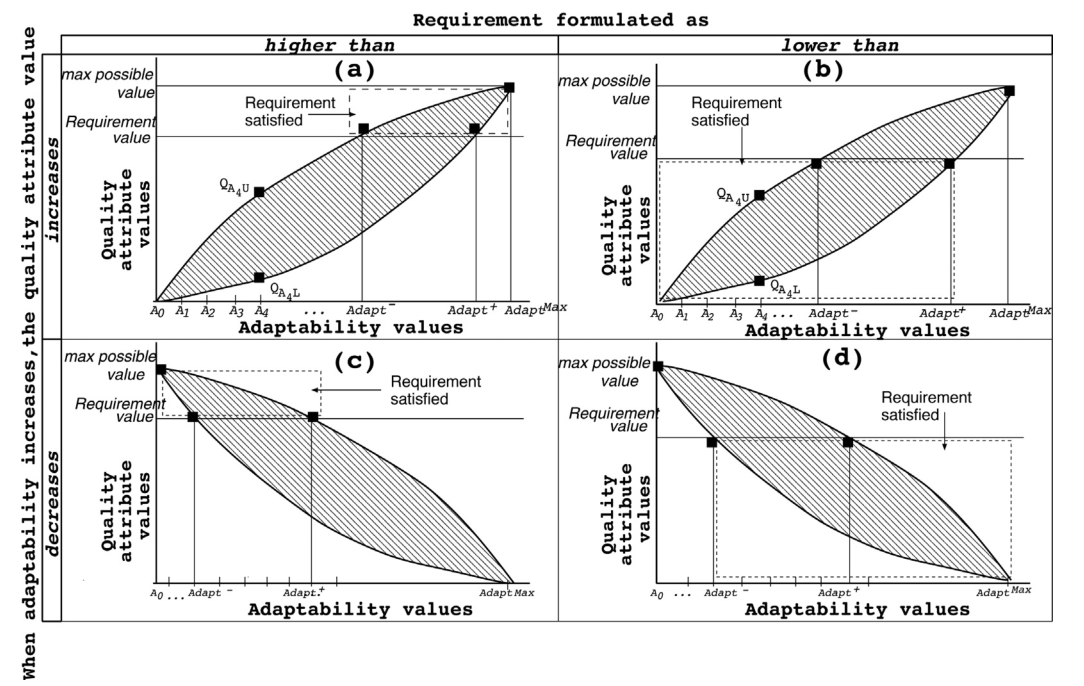
\includegraphics[scale=0.55]{img/solar-inter-cases.png}}
	\caption[Relations among adaptability and other quality attributes.]{Relations among adaptability and other quality attributes.\cite{solar}}
	\label{fig:solar-inter-cases}
\end{figure} 
\subsection{Analysis of the approach and its limits}
Both of these tools want to help the software architect in choosing the right set of components in order to satisfy the adaptability requirements and if possible other quality attributes. With the SOLAR framework all the possible architectures that satisfy the requisites are generated and the choice is left to the architect. This approach is for sure slower but is a valid tool to have an idea of the possible outcome and build an architecture from scratch. On the other side it presents some limitations presented in no particular order:
\begin{itemize}
	\item It analyzes all the architecture only with a static analysis using the component diagram.
	\item All components are given equal importance thus the time a component is used and the number of usages per call is completely ignored.
	\item It does not considers the probability of failure of a component at runtime.
	\item Requires a lot of time to produce complete results.
\end{itemize}
In the next chapter it is shown how to analyze the quality of a software and in particular how to evaluate the adaptability of a software with respect to some attributes such as cost and availability.
\chapter{The new quality metrics}
\label{cap:quality-metrics}
In this chapter it is explained how to improve the SOLAR framework in order to integrate the existing metrics with another set of metrics in order to provide the software engineer with more information regarding the architecture he's building. 

All modern applications are born to meet some functional requirements that often are subject to changes due to the fact that the environment where they operate is dynamic and can change in a unpredictable way. In the academic and industrial reality rose up the need to standardize some quality metrics in order to evaluate a software, this is the case of the \textbf{ISO/IEC 25010} standard called \emph{Systems and software Quality Requirements and Evaluation (SQuaRE)}\cite{iso/iec-25010}. However in the self-adaptive context these metrics are not of much help since they do not account the ability of these systems to auto adapt whenever they need it.

To overcome this problem some more new metrics have been defined that analyze the architecture in two different ways:
\begin{itemize}
	\item using a component diagram as defined in the UML standard\cite{uml} to analyze the static behavior
	\item using a sequence diagram as defined in the UML standard\cite{uml} to analyze the runtime behavior
\end{itemize}

The final objective is to define some adaptability metrics for the architecture as a whole and for every service that the architecture uses. In a more specific way what is shown is how important is every service in a architecture and as a consequence, how important is every component.

\section{Systems and software Quality Requirements and Evaluation}
\label{sec:square}
\textbf{ISO/IEC 25010}, \emph{Systems and software engineering — Systems and software Quality Requirements and Evaluation (SQuaRE)}\cite{iso/iec-25010} is an international standard for the evaluation of software quality that replaced the previous \textbf{ISO/IEC 9126} \emph{Software engineering — Product quality standard}\cite{iso/iec-9126}.

It presents eight product quality characteristics (in contrast to ISO 9126's six):
\begin{itemize}
	\item Functional suitability - degree to which a product or system provides functions that meet stated and implied needs when used under specified conditions
	\item Reliability - degree to which a system, product or component performs specified functions under specified conditions for a specified period of time
	\item Usability - degree to which a product or system can be used by specified users to achieve specified goals with effectiveness, efficiency and satisfaction in a specified context of use
	\item Performance efficiency - performance relative to the amount of resources used under stated conditions
	\item Maintainability - degree of effectiveness and efficiency with which a product or system can be modified by the intended maintainers
	\item Portability - degree of effectiveness and efficiency with which a system, product or component can be transferred from one hardware, software or other operational or usage environment to another
	\item Compatibility - degree to which a product, system or component can exchange information with other products, systems or components, and/or perform its required functions, while sharing the same hardware or software environment
	\item Security - degree to which a product or system protects information and data so that persons or other products or systems have the degree of data access appropriate to their types and levels of authorization
\end{itemize}

\section{The New Metrics}
\label{sec:new-metrics}
All the metrics shown in this section are focused on two primary quality attributes for the software engineer which are \emph{availability} and \emph{cost}. As a consequence two parameters must be given to perform some of the calculations:
\begin{itemize}
	\item \emph{$availability_{target}$} which represent the minimum availability the system must have
	\item \emph{$cost_{target}$} which represents the maximum cost the system must have
\end{itemize}
Both this parameters are given by the software engineer and come from the previous analysis of the requisites.

In table \ref{tab:new-metrics-summary} are summarized all the terms used in the equations.

\begin{table}[ht!b]
	\centering
	\begin{tabular}{|l|l|}
		\hline
		\multicolumn{1}{|c|}{Name} & \multicolumn{1}{c|}{Meaning} \\
		\hline 
		$availability_{target}$ & represent the minimum availability the system must have \\
		\hline
		$cost_{target}$ & represents the maximum cost the system must have \\ 
		\hline
		$C_i$ & Component \emph{i} \\ 
		\hline
		$T_{C_i}$ & Execution time for component \emph{i} \\
		\hline
		$PS_i$ & Provided service \emph{i} \\
		\hline
		$N_{exec_{PS_i}}$ & Number of executions of provided service \emph{i} \\
		\hline
		$T_{PS_i}$ & Execution Time of provided service \emph{i} \\
		\hline
		$TotTime$ & Total time of execution \\
		\hline
		$S_i$ & Service \emph{i} \\
		\hline
		$T_{S_i}$ & Execution time of service \emph{i} \\
		\hline
		$N_{exec_{S_i}}$ & Number of executions of service \emph{i} \\
		\hline
		$P_{exec_{S_i}}$ & Probability of execution service \emph{i} \\
		\hline
		$ExecPerCall_{S_i}$ & Number of execution per call of service \emph{i} \\
		\hline
		$N_{exec_{PS_i}}$ &  Number of executions of provided service \emph{i} \\
		\hline
		$TimeAction_{S_i}$ & The time a service \emph{i} is working \\
		\hline
		$AV_{C_i}$ & Intrinsic availability of component \emph{i} \\
		\hline
	\end{tabular} 
	\caption[New Metrics]{Summary of the metrics.}
	\label{tab:new-metrics-summary}
\end{table}

\subsection{Components}
\subsubsection{Fitness ratio w.r.t. availability}
This metric defines the ratio between a component availability and the target system availability. This result is from the hypothesis that a component with a high availability can provide, at first glance, more guarantees of functioning. 
\[ FRA_{C_i} \in \mathbb{R}^+_0 \; | \; FRA_{C_i} = \frac{1 - availability_{target}}{1- availability_{C_i}} \]

This means that if the result is $\ge 1$ the component satisfies the target requisite and as a consequence it can work for a longer time improving the availability of the service it offers. 

A value $\ge 0 $ and $<1$ indicates that this component is prone to failure more frequently than how is requested in the architecture.

\subsubsection{Fitness ratio w.r.t. cost}
Defines the ratio between a component cost and the system target cost. 

\[ FRC_{C_i} \in \mathbb{R}^+_0 \; | \; FRC_{C_i} = \frac{cost_{target}}{cost_{C_i}}\]

With the same component cost, if the system target cost grows higher the Fitness Ratio w.r.t. Cost becomes bigger. This implies that the bigger the component and the system target cost gap is, the more can be saved from buying this component w.r.t. the maximum budget invested in buying all the components.

\subsubsection{Weight of residence time}
Calculates which fraction of time a component is running w.r.t total running time of the architecture.

\[ T_{C_i} \in \mathbb{R}^+ \; | \; T_{C_i} = \sum_{i=0}^{n} N_{exec_{PS_i}} * T_{PS_i} \]

\[ TotTime \in \mathbb{R^+} \; | \; TotTime = \sum_{i=0}^{n}N_{exec_{S_i}} * T_{S_i} \]

\[ WRT \in \mathbb{R}^+ \; | \; WRT = \frac{T_{C_i}}{TotTime} \]

Higher results means that the component runs more than others, thus is a important piece of the architecture. A failure in this component can compromise the functioning of the architecture in a bigger way than a failure of other components.

\subsection{Services}
\subsubsection{Number of executions}
Defines the number of times a service is executed.

\[ N_{exec_{S_i}} \in \mathbb{N} \; | \; \forall PS_i \;\, N_{exec_{S_i}} = \sum_{i=0}^{n} P_{exec_{S_i}} * ExecPerCall_{S_i} * N_{exec_{PS_i}} \]

\subsubsection{Probability to be running}
Defines the probability that a given service is running in a given moment.

\[ PTBR_{S_i} \in [0..1] \; | \; PTBR_{S_i} =  \frac{{N_{exec_{S_i}}}}{ \sum_{i=0}^{n}  N_{exec_{S_i}}} \]

\subsubsection{In Action}
This metrics calculates the probability to find a given service active considering the dynamic analysis of the architecture.

\[ TimeAction_{S_i} \in \mathbb{R}^+ \; | \; \sum_{j=0}^{n} T_{exec{S_i}Path_j} * P_{exec_{S_i}} \]
\[ InAction_{S_i} \in [0..1] \; | \; InAction_{S_i} = \frac{TimeAction_{S_i}}{{\sum_{i=0}^n}TimeAction_{S_i}} \]

It considers all the possible paths available in the selected workflow; in this way a workflow with an \texttt{Alt} and/or \texttt{Opt} block in the sequence diagram can be represented in a correct way.

\subsection{Architecture}
\subsubsection{Global availability of system}
Defines the availability of the components that are in the architecture as a probability that are all active in a given instant.
\[ GAS \in \mathbb{R}^+_0 \; | \; \forall C_i \; GAS = \prod_{i=0}^{n} FRA_{C_i} \]
A better availability of a component in the architecture implies a better Fitness Ratio w.r.t. Availability that is reflected in a better global availability. Higher numbers mean better availability.
\subsubsection{Global cost of system}
Defines the total cost of the components in an architecture w.r.t. the cost of each individual component.
\[ GCS \in \mathbb{R}^+_0 \; | \; \forall C_i GCS = \sum_{i=0}^{n} FRC_{C_i} \]
\subsubsection{Total Static Availability}
This methods calculate the Availability of an architecture without considering actual workflows of the architecture, so it uses the component diagram. It considers all components as used and considers a call to the main service to use always all the components.

Given that $S_x$ is the main offered service we can calculate the availability of such service as total availability of the system.
\begin{itemize}
\item If a component is terminal, so doesn't require any service:
\[ Av(C_{i}) \in \mathbb{R}^+_0 \; | \; Av(C_{i}) = AV_{C_{i}} \]
\item  If a component is not terminal and requires some service $S_k$:
\[ Av(C_{i}) \in \mathbb{R}^+_0 \; | \; \forall S_k \; Av(C_{i}) = AV_{C_{i}}*\prod_{k=0}^{n} ((1-p_{S_k}^{C_{i}}) + p_{S_k}^{C_{i}} * (AV_{S_k})^{N_{S_k}^{C_i}}) \]
\end{itemize}
With these we can calculate the availability of $S_x$ thus the availability of the architecture with $C_i$ being any component that offers $S_x$.
\[ Av(S_x) \in \mathbb{R}^+_0 \; | \; \exists C_i \; Av(S_x) = 1-\prod_{i=0}^{n}(1-Av_{C_i}) \]

\chapter{The Adaptability Analyzer Software}
\label{cap:design}

To provide the software engineer a tool that can ease his work a new software has been developed ad hoc, called Adaptability Analyzer Tool.

This tool has been developed from scratch with some goals in mind and puts together the previous SOLAR\cite{solar} metrics with the new metrics presented in Chapter \ref{cap:quality-metrics}. All the goals are explained in the following section.

\section{Adapt Analyzer Goals}
\subsection{User Point of View}
From a usability point of view the first goal of this software was to be a tool that can be used by every software engineer without knowing the underlying programming language or how the code is structured; to achieve this I've chosen to provide the software with a Graphical User Interface (GUI) that doesn't require any programming skill to be used.

Another goal was that creating an architecture and then perform calculations should be made easy for everyone, not only for the software engineer, so every result is clearly visible in the GUI and, where possible, numeric results are supported by Cartesian graphs and/or visual representations.

How these goal are achieved is explained in the following section.
\subsection{Programmer Point of View}
From a programming point of view, instead, the software has to be portable so it can be run on most computers, without strict limitations on operating systems and/or hardware. This is achieved by using the Java programming language\cite{java-se}. 

With this programming language the choice on how to develop the GUI were only two framework (discarding the old AWT\cite{awt}): Swing\cite{swing} or JavaFX\cite{javafx}. I've chosen to use the newer JavaFX because it should become the new standard for developing Java applications and it provides a set of useful API to the scope of this software.

Others programming goals were to provide a software that can have a small memory footprint and low CPU usage but that can provide results in a meaningful time frame; this is achieved by using common design patterns with efficient algorithms in term of time and memory complexity.

The last goal was to make the user be able to export and import his architecture, thus interrupting and resuming his work on another machine is made easy; this is accomplished by serializing the architecture in JSON files.

More details on programming choices can be found in the Appendix \ref{app:usermanual}



\chapter{Experimental Evaluation}
\label{cap:evaluation}

In this chapter the Adaptability Analyzer Software is used to study two main cases: one is the Tele Assistance System\cite{teleassist} and the other one is generated with the integrated Architecture Generator.

\section{Tele Assistance: A Self-Adaptive Service-Based System}
Tele Assistance System, also known as TAS, is a research, done by the Universities of Linnaeus and York  \cite{teleassist}, on self-adaptation in the domain of service-based systems. Originally introduced in \cite{valid-web-serv} has already been used in the evaluation of several self-adaptation solutions \cite{valid-web-serv}, \cite{sas-quant-ver}, \cite{dyn-qos-manage}, \cite{mod-evo-conf}, \cite{conq-compl}, albeit based on ad-hoc implementations, scenarios and evaluation metrics that make the comparison of these solutions and its use to evaluate other solution very difficult. It is an official examplar and it is available via the SEAMS exemplar website: \url{http://self-adaptive.org/exemplars/tas}.

To address these limitation the University of York implemented TAS on their Research Service Platform (ReSeP) in conjunction with concrete scenarios in order to have an immediate use in evaluation of the self-adaptation solutions.

The system provides health support to chronic condition sufferers within the comfort of their homes. TAS uses a combination of sensors embedded in a wearable device and remote services from healthcare, pharmacy and emergency service providers. As shown in Figure \ref{fig:tas-workflow}, the TAS workflow takes periodical measurements of the vital parameters of a patient and employs a third-party medical service for their analysis. The analysis result may trigger the invocation of a pharmacy service to deliver new medication to the patient or to change his/her dose of medication, or the invocation of an alarm service leading, e.g., to an ambulance being dispatched to the patient. The same alarm service can be invoked directly by the patient, by using a panic button on the wearable device.

\begin{figure}[ht]
	\centerline
	{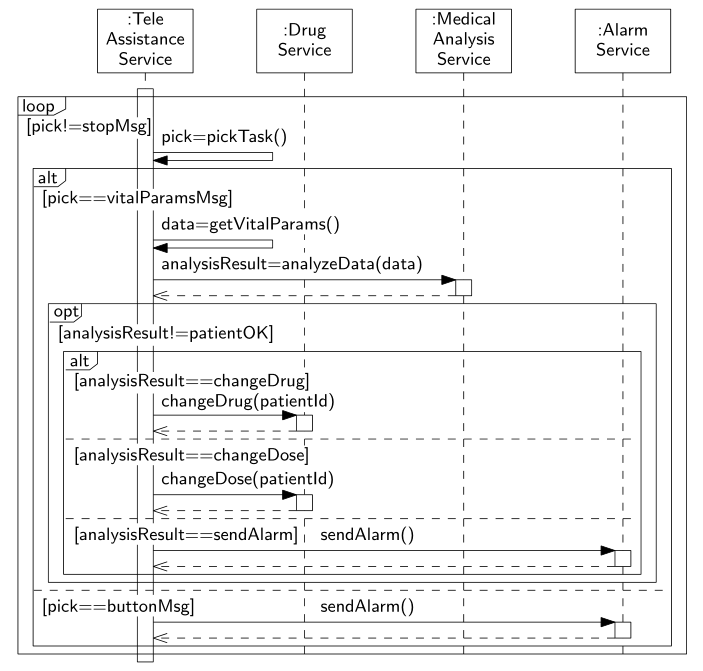
\includegraphics[scale=0.55]{img/tas-workflow.png}}
	\caption[TAS Workflow]{TAS workflow\cite{teleassist}.}
	\label{fig:tas-workflow}
\end{figure}

They also provide some generic adaptation scenarios shown in Table \ref{tab:tas-scenarios} and some metrics shown in table \ref{tab:tas-metrics}

In conclusion TAS is a reference implementation of a service based system and generic adaptation scenarios associated with different types of uncertainty. First, it aims to promote research and understanding among multiple researchers and research groups, through enabling the comparison of different self-adaptation approaches, without favoring any particular approach. Second, TAS aims to serve the advance of single research efforts by reducing the time required to evaluate self-adaptation solutions. Finally, it aims to contribute to advancing the practice of engineering self-adaptive systems, by being a realistic example of a widely used type of software system.

\begin{table}[ht!b]
	\centering
	\begin{tabular}{|l|p{3.5cm}|p{3.5cm}|p{3.5cm}|}
		\hline 
		\textbf{Scenario} & \textbf{Type of uncertainty} & \textbf{Type of adaptation} & \textbf{Type of requirements}  \\
		\hline 
		S1 & Unpredictable environment: service failure  & Switch to equivalent service; Simultaneous invocation of several services for idempotent operation & QoS: Reliability, cost \\
		\hline 
		S2 & Unpredictable environment: variation of service response time & Switch to equivalent service; Simultaneous invocation of several services for idempotent operation & QoS: Performance, cost \\
		\hline 
		S3 & Incomplete information: new service & Use new service & QoS: Reliability, performance, cost \\ 
		\hline 
		S4 & Changing requirements: new goal & Change workflow architecture; Select new service of the change on the levels & Functional: new operation \\ 
		\hline 
		S5 & Inadequate design: wrong operation sequence & Change workflow architecture & Functional: operation sequence compliance \\ 
		\hline
		
	\end{tabular} 
	\caption[TAS Scenarios]{Generic adaptation scenarios for service-based systems\cite{teleassist}.}
	\label{tab:tas-scenarios}
\end{table}

\begin{table}[ht!b]
	\centering
	\begin{tabular}{|p{3cm}|p{10cm}|}
		\hline 
		\textbf{Quality Attribute} & \textbf{Metrics} \\ 
		\hline 
		Reliability & Number of failed service invocations
		Number of specific operation sequence failures
		Mean time to recovery \\ 
		\hline 
		Performance & Number of specific operation sequences exceeding allowed execution time \\ 
		\hline 
		Cost & Cumulative service invocation cost over given time period \\ 
		\hline 
		Functionalities & Number of faulty process executions \\ 
		\hline 
		
	\end{tabular} 
	\caption[TAS Metrics]{Quality attributes and metrics for the evaluation and comparison of SBS self-adaptation solutions\cite{teleassist}.}
	\label{tab:tas-metrics}
\end{table}

In the Adapt Analyzer tool as been implemented the scenario S1 presented in Table \ref{tab:tas-scenarios} which considers equivalent services that differ one another in some of their characteristics and qualities.

\clearpage

\subsection{Adaptability Analyzer Results}

To recreate the original Tele Assistance System in the tool, the architecture has been divided in multiple components, each offering or requesting the services presented in the original system as shown in Table \ref{tab:tas-original-services}. All the values in Table \ref{tab:tas-original-services} are taken from the official exemplar \cite{teleassist}.

\begin{table}[ht!b]
	\centering
	\begin{tabular}{|p{5cm}|p{3cm}|p{1cm}|}
		\hline 
		\textbf{Service Name} & \textbf{Failure Rate} & \textbf{Cost} \\ 
		\hline 
		Alarm Service 1 & 0.11 & 4.0 \\
		\hline 
		Alarm Service 2 & 0.04 & 12.0 \\ 
		\hline 
		Alarm Service 3 & 0.18 & 2.0 \\ 
		\hline 
		Medical Analysis Service 1 & 0.12 & 4.0 \\ 
		\hline
		Medical Analysis Service 2 & 0.07 & 14.0 \\ 
		\hline
		Medical Analysis Service 3 & 0.18 & 2.0 \\ 
		\hline
		Drug Service 1 & 0.01 & 5.0 \\ 
		\hline
		
	\end{tabular} 
	\caption[TAS Services]{Tele Assistance Services in the original formulation.}
	\label{tab:tas-original-services}
\end{table}

Therefore the components are divided in three main groups each offering a service between Alarm, Medical Analysis and Drug Service and one more component is added to recreate the entry point of the original system. Since the main component is not specified in the original system, I have created a plausible component with its parameters called \emph{TA}. In Table \ref{tab:tas-comp} are visible all the components and Figure \ref{fig:tas-arch} is a visual representation of the architecture generated with the tool.

\begin{table}[ht!b]
	\centering
	\begin{tabular}{|p{3cm}|p{2.5cm}|p{1cm}|}
		\hline 
		\textbf{Component Name} & \textbf{Availability} & \textbf{Cost} \\ 
		\hline 
		AS1 & 0.90 & 4.0 \\
		\hline 
		AS2 & 0.96 & 12.0 \\ 
		\hline 
		AS3 & 0.85 & 2.0 \\ 
		\hline 
		MAS1 & 0.89 & 4.0 \\ 
		\hline
		MAS2 & 0.93 & 14.0 \\ 
		\hline
		MAS3 & 0.85 & 2.0 \\ 
		\hline
		DS 1 & 0.99 & 5.0 \\ 
		\hline
		TA & 0.9 & 5.0 \\ 
		\hline
		
	\end{tabular} 
	\caption[TAS Components]{Tele Assistance Components as they are represented in the tool.}
	\label{tab:tas-comp}
\end{table}
In Table \ref{tab:tas-serv} are presented the components with the associated services and their parameters. Since every service is likely called as much as the other all the Required Services have a Used Probability of $ \frac{1}{3} $. All the other parameters are made up in order to make the tool work because the exemplar doesn't provide them. Also the TA service is not specified in the original formulation of the system.
\begin{table}[ht!b]
	\centering
	\begin{tabular}{|p{2cm}|p{2.5cm}|p{1.4cm}|p{1.7cm}|p{1.5cm}|p{1.8cm}|}
		\hline 
		\textbf{Component} & \textbf{Service Name} & \textbf{Type of Service} & \textbf{Execution Time} & \textbf{Used Probability} & \textbf{Number of Execution per Call} \\ 
		\hline 
		AS1 & Alarm & Provided & 1.0 & & \\
		\hline 
		AS2 & Alarm & Provided & 5.0 & & \\
		\hline 
		AS3 & Alarm & Provided & 2.0 & & \\
		\hline 
		MAS1 & MedicalAnalysis & Provided & 5.0 & & \\ 
		\hline
		MAS2 & MedicalAnalysis & Provided & 10.0 & & \\ 
		\hline
		MAS3 & MedicalAnalysis & Provided & 20.0 & & \\ 
		\hline
		DS 1 & Drug & Provided & 10.0 & & \\
		\hline
		\multirow{4}{*}{TA} & Alarm & Required & & 0.33 & 1 \\
		& Drug & Required & & 0.33 & 1 \\
		& MedicalAnalysis & Required & & 0.33 & 1 \\\cline{2-6}
		& TeleAssistance & Provided & 1 & & \\
		\hline
		
	\end{tabular} 
	\caption[TAS Service]{Tele Assistance Components with their associated services.}
	\label{tab:tas-serv}
\end{table}

\begin{figure}[ht]
	\centerline
	{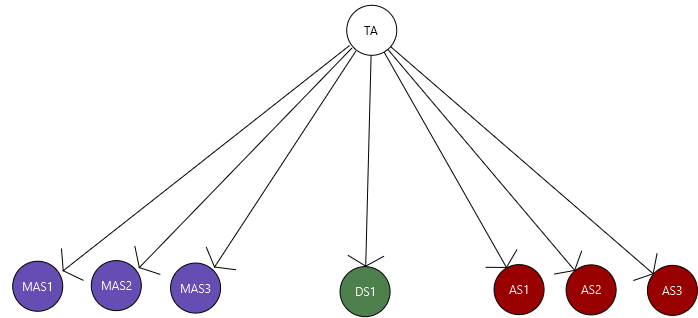
\includegraphics[scale=0.55]{img/TeleAssistance.png}}
	\caption[TAS Architecture]{TAS Architecture generated by the tool.}
	\label{fig:tas-arch}
\end{figure}

To test the architecture, a workflow has been created that reflects part of the original sequence diagram shown in Figure \ref{fig:tas-workflow}. This workflow provides two cases:
\begin{itemize}
	\item The service is invoked and after having read the vital parameters and analyzed the data launches an alarm.
	\item The service is invoked and after having read the vital parameters and analyzed the data changes the drug that is currently administered to the patient.
\end{itemize}

The original formulation provides five possible paths but only two are presented in this evaluation. This choice has been done since \texttt{Alt} and \texttt{Opt} blocks can't be nested in the actual implementation.

In Figure \ref{fig:tas-path1} and \ref{fig:tas-path2} is shown how the two workflows are implemented in the tool with respect to the original Sequence Diagram \ref{fig:tas-workflow}, with the unused parts removed to reduce clutter.

\clearpage
\subsubsection{Path 1}
\begin{figure}[ht]
	\centerline
	{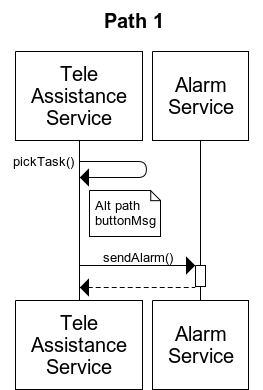
\includegraphics[scale=0.6]{img/TeleAssistanceOrigPath1.png}}
	\caption[TAS Original Workflow Path Alarm]{TAS original workflow with the alarm path selected.}
	\label{fig:tas-or-path1}
\end{figure}

\begin{figure}[ht]
	\centerline
	{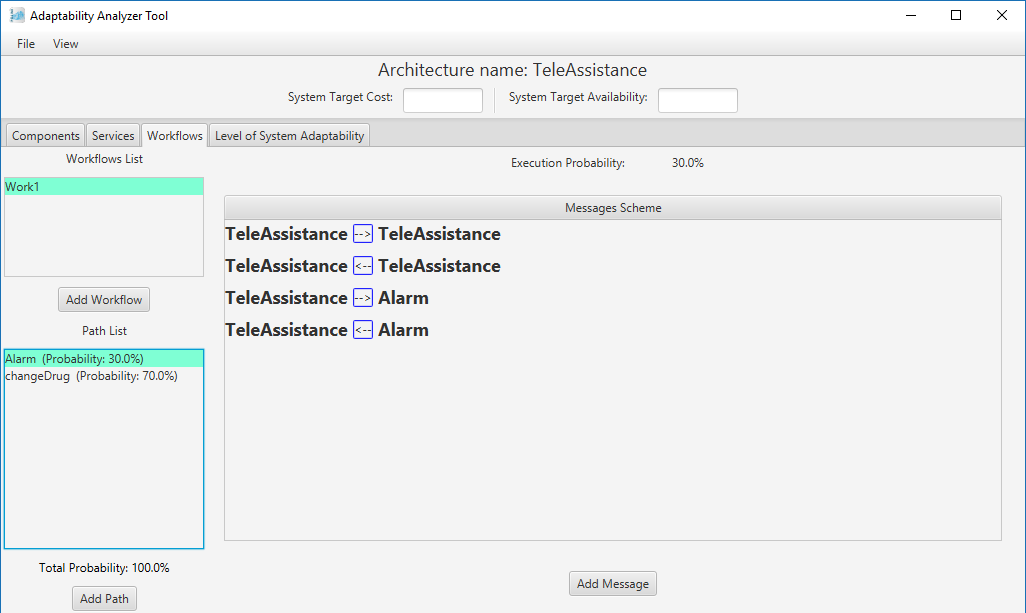
\includegraphics[scale=0.55]{img/TeleAssistancePath1.png}}
	\caption[TAS Workflow Path Alarm]{TAS workflow with the alarm path selected.}
	\label{fig:tas-path1}
\end{figure}

\clearpage
\subsubsection{Path 2}

\begin{figure}[ht]
	\centerline
	{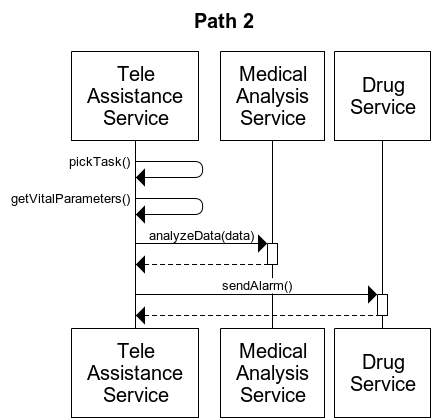
\includegraphics[scale=0.55]{img/TeleAssistanceOrigPath2.png}}
	\caption[TAS Original Workflow Path Alarm]{TAS original workflow with the changeDrug path selected.}
	\label{fig:tas-or-path2}
\end{figure}

\begin{figure}[ht]
	\centerline
	{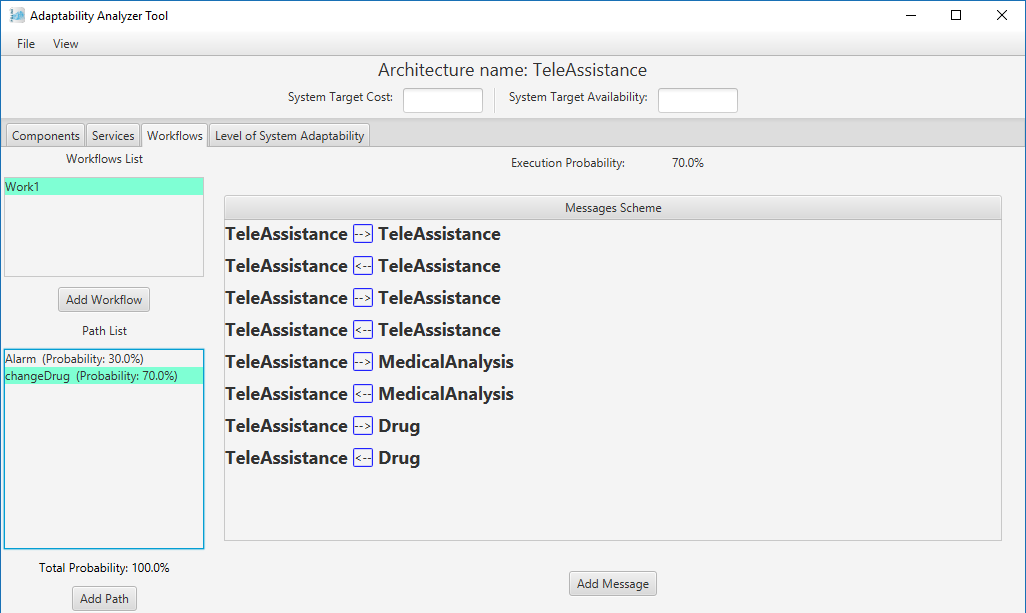
\includegraphics[scale=0.55]{img/TeleAssistancePath2.png}}
	\caption[TAS Workflow Path changeDrug]{TAS workflow with the changeDrug path selected.}
	\label{fig:tas-path2}
\end{figure}

\clearpage

After performing some calculation with the Adaptability Analyzer Tool, with \emph{System Target Cost} set to 50 and \emph{System Target Availability} set to 0.9, on this architecture the following result are achieved:

\begin{table}[ht!b]
	\centering
	\begin{tabular}{|l|c|}
		\hline
		Metric & Measure \\
		\hline 
		\textbf{Global FRA} & 12.53 \\ 
		\hline 
		\textbf{Global FRC} & 102.74 \\
		\hline 
		\textbf{Total Static Availability} & 0.90 \\
		\hline 
		\textbf{Total Cost} & 48.00 \\
		\hline 
		\textbf{Mean of Absolute Adaptability} & 2.00 \\
		\hline
		\textbf{Mean of Relative Adaptability} & 1.00 \\
		\hline
		\textbf{Level of System Adaptability} & 1.00 \\
		\hline
	\end{tabular} 
	\caption[TAS Service Architecture Metrics]{Tele Assistance Architecture metrics results.}
	\label{tab:tas-arch-res}
\end{table}

\begin{table}[ht!b]
\centering
\begin{threeparttable}
	\begin{tabular}{|l|c|c|c|}
		\hline 
		\textbf{Component} & \textbf{FRA}\tnote{1} & \textbf{FRC}\tnote{2} & \textbf{WRT}\tnote{3} \\ 
		\hline 
		AS1 & 0.91 & 12.50 & 0.02 \\
		\hline 
		AS2 & 2.50 & 4.17 & 0.09 \\
		\hline 
		AS3 & 0.83 & 25.00 & 0.04 \\
		\hline 
		MAS1 & 0.83 & 12.50 & 0.09 \\
		\hline
		MAS2 & 1.43 & 3.57 & 0.18 \\
		\hline
		MAS3 & 0.56 & 25.00 & 0.36 \\
		\hline
		DS1 & 10.00 & 10.00 & 0.18 \\
		\hline
		TA & 1 & 10.00 & 0.05 \\
		\hline
	\end{tabular}
	\begin{tablenotes}\footnotesize
		\item[1] Fitness Ratio w.r.t. Availability. See: \ref{met:fra}
		\item[2] Fitness Ratio w.r.t. Cost. See: \ref{met:frc}
		\item[3] Fitness Ratio w.r.t. Availability. See: \ref{met:wrt}
	\end{tablenotes}
\end{threeparttable}
\caption[TAS Service Components Metrics]{Tele Assistance Components metrics results.}
\label{tab:tas-comp-res}
\end{table}

\begin{table}[ht!b]
	\centering
	\begin{tabular}{|l|c|c|c|c|}
		\hline 
		\multirow{2}{*}{\textbf{Service}} & \textbf{Number} & \textbf{Probability to} & \textbf{Absolute} & \textbf{Relative} \\ 
		& \textbf{of Executions} & \textbf{be running} & \textbf{Adaptability} & \textbf{Adaptability} \\
		\hline 
		Alarm & 0.33 & 0.17 & 3 & 1 \\
		\hline 
		Drug & 0.33 & 0.17 & 1 & 1 \\
		\hline 
		MedicalAnalysis & 0.33 & 0.17 & 3 & 1 \\
		\hline 
		TeleAssistance & 1 & 0.5 & 1 & 1 \\
		\hline
	\end{tabular} 
	\caption[TAS Service Services Metrics]{Tele Assistance Services metrics results.}
	\label{tab:tas-serv-res}
\end{table}

As expected from Table \ref{tab:tas-arch-res} can be seen that the Architecture has a high value for Global Fitness Ratio w.r.t. Cost, this means that every component costs very little with respect to the target cost; on the other hand, Global FRA does not inform the architect that only one component has a much better availability than the one requested for the system. 

All the other informations are basic information about the architecture and, in the case of the Total Static Availability, how it behaves from a static point of view.

From Table \ref{tab:tas-comp-res} it can be seen that, as expected, all the components that respect the targets imposed by the architect have values $>1$. The Weight Residence Time shows which is the probability that a component is currently working with respect to the total time from a static point of view.

Table \ref{tab:tas-serv-res} shows how service behaves in the architecture; since all of them, excluding TeleAssistance that is the service that the final user utilizes, are equally probable thus for every call the Number of Executions is 0.33 or $\frac{1}{3}$. The Probability to be Running highlights the fact that since half of the computation is done by the main TeleAssistance service the other half is done for the effective used service thus every service has a probability to be working of 0.17 or $\frac{1}{6}$.

The last two columns show how much the component is replicated and if all the replication are used, so the Alarm and MedicalAnalysis which are replicated three times have an Absolute Adaptability of 3, instead the TeleAssistance and Drug service which are not replicated have an Absolute Availability of 1; in this architecture all the component are used all the services have a Relative Adaptability of 1, since the Relative Adaptability is calculated as $\frac{usedComponents}{components}$.

Lets focus now on the dynamic analysis and take a look to the drug service; using the workflow shown in Figures \ref{fig:tas-path1} and \ref{fig:tas-path2} the drug service has a \emph{InAction} and Service Availability of 0.21. Such a low availability is due to the fact that the Drug Service is provided by only one component in the provided workflow.

The \emph{InAction} metric shows that in the particular case of the selected workflow the probability that the drug service is active is higher than the static analysis since in the workflow it is used in the \emph{Path 2} and in the same path the Alarm Service is not used. The service availability is equal to the \emph{InAction} metric; this is just a case and a rounding issue since the drug service has an availability that is almost 1.

The results provided by the tool provide some useful information to the Software Architect from which he can come to some conclusions; in this case, for example, it is clear that the \emph{MAS3} component despite having the lowest cost, it also have the lowest availability and higher execution time that can impact negatively on the overall performance of the system, so instead of buying a \emph{MAS3} component, he should buy two \emph{MAS2} components that costs a little more and provide better performance and availability. Another useful information can be that the \emph{TA} component is critical since it is the entry point of the system, losing such component makes the entire system unavailable.

On the adaptability point of view we can examine the graph in Figure \ref{fig:tas-adapt} for a value of adaptability of 0.75. With this level of adaptability all services can be provided to the final user but with very different costs:
\begin{itemize}
	\item \textbf{Cost = 22:} we use components AS1, AS3, DS1, MAS1, MAS2 and TA; lower cost but low performance if we relate to the component specifications.
	\item \textbf{Cost = 44:} we use components AS1, AS2, DS1, MAS1, MAS2 and TA; higher cost but also better performance than before.
\end{itemize}


\begin{figure}[ht]
	\centerline
	{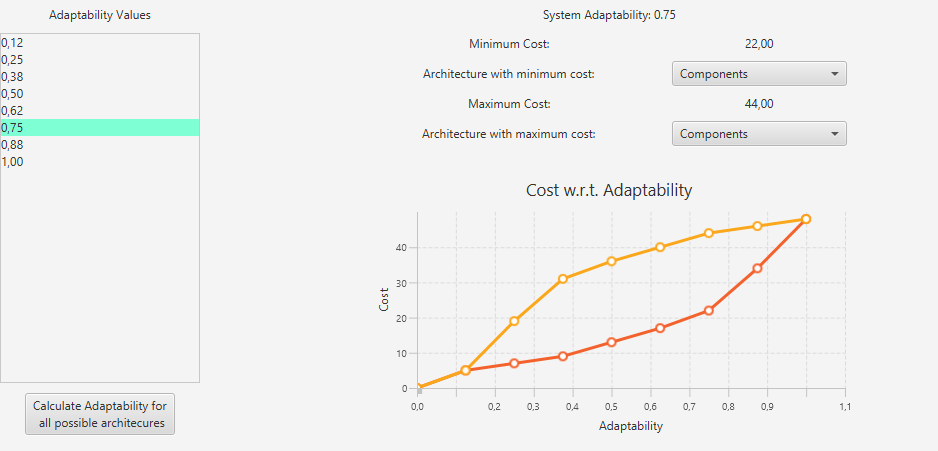
\includegraphics[scale=0.55]{img/tas-adapt.png}}
	\caption[TAS Graph showing Adaptability]{TAS Graph showing Adaptability.}
	\label{fig:tas-adapt}
\end{figure}

The graph also shows how different are the costs at the same adaptability level, the software architect can thus have a better overview over the system and its components.
\clearpage

\section{Generic Generated Study Case}
To show the powerfulness of this tool and its generator, another generic generated architecture has been analyzed and its shown in Figure \ref{fig:testarch} and Tables \ref{tab:ag-comp} and \ref{tab:ag-serv}. 

This architecture has been evaluated to see how well the tool can perform even with more complicated systems than the Tele-Assitance exemplar; in the architecture schema shown in Figure \ref{fig:testarch} is immediately visible that the components call each other in a chain and some of them are replicated more than other. This implies that the calculations to perform the evaluation are more computationally elaborated than in the previous case, especially the adaptability of the system that grows exponentially in time with respect to the number of components and branches.

\begin{figure}[ht]
	\centerline
	{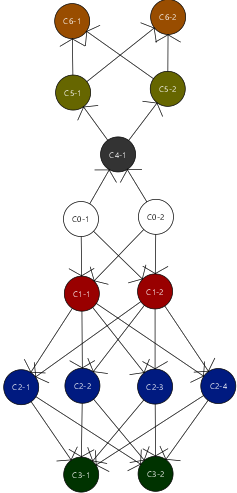
\includegraphics[scale=0.9]{img/autogenerated_arch.png}}
	\caption[Generic Generated Architecture]{An architecture generated by the tool generator.}
	\label{fig:testarch}
\end{figure}

\begin{table}[ht!b]
	\centering
	\begin{tabular}{|p{2cm}|p{2cm}|p{1cm}||p{2cm}|p{2cm}|p{1cm}|}
		\hline 
		\textbf{Component Name} & \textbf{Availability} & \textbf{Cost} & \textbf{Component Name} & \textbf{Availability} & \textbf{Cost} \\ 
		\hline 
		C0-1 & 0.90 & 33.0 & C3-1 & 0.90 & 1.0 \\
		\hline 
		C0-2 & 0.87 & 20.0 & C3-2 & 0.99 & 10.0 \\ 
		\hline 
		C1-1 & 0.90 & 5.0 & C4-1 & 0.90 & 15.0 \\ 
		\hline 
		C1-2 & 0.93 & 7.0 & C5-1 & 0.85 & 6.0 \\ 
		\hline
		C2-1 & 0.60 & 10.0 & C5-2 & 0.90 & 10.0 \\ 
		\hline
		C2-2 & 0.99 & 60.0 & C6-1 & 0.83 & 20.0 \\ 
		\hline
		C2-3 & 0.30 & 5.0 & C6-2 & 0.90 & 100.0 \\ 
		\hline
		C2-4 & 0.87 & 20.0 & & & \\ 
		\hline
	\end{tabular} 
	\caption[TAS Components]{Tele Assistance Components as they are represented in the tool.}
	\label{tab:ag-comp}
\end{table}

\begin{table}[ht!b]
	\centering
	\begin{tabular}{|p{2cm}|p{2.3cm}|p{1.4cm}|p{1.7cm}|p{1.5cm}|p{1.8cm}|}
		\hline 
		\textbf{Component} & \textbf{Service Name} & \textbf{Type of Service} & \textbf{Execution Time} & \textbf{Used Probability} & \textbf{Number of Execution per Call} \\ 
		\hline 
		\multirow{3}{*}{C0-1} & S0 & Provided & 1.0 & & \\\cline{2-6}
		& S1 & Required & & 0.90 & 3 \\
		& S4 & Required & & 0.30 & 1 \\
		\hline 
		\multirow{3}{*}{C0-2} & S0 & Provided & 2.0 & & \\\cline{2-6}
		& S1 & Required & & 0.90 & 1 \\
		& S4 & Required & & 0.10 & 10 \\
		\hline 
		\multirow{2}{*}{C1-1} & S1 & Provided & 2.0 & & \\\cline{2-6}
		& S2 & Required & & 0.90 & 4 \\
		\hline 
		\multirow{2}{*}{C1-2} & S1 & Provided & 1.0 & & \\\cline{2-6}
		& S2 & Required & & 0.90 & 1 \\
		\hline
		\multirow{2}{*}{C2-1} & S2 & Provided & 1.0 & & \\\cline{2-6}
		& S3 & Required & & 0.90 & 1 \\
		\hline
		\multirow{2}{*}{C2-2} & S2 & Provided & 4.0 & & \\\cline{2-6}
		& S3 & Required & & 0.50 & 1 \\
		\hline
		\multirow{2}{*}{C2-3} & S2 & Provided & 9.0 & & \\\cline{2-6}
		& S3 & Required & & 0.50 & 3 \\
		\hline
		\multirow{2}{*}{C2-4} & S2 & Provided & 1.0 & & \\\cline{2-6}
		& S3 & Required & & 0.70 & 1 \\
		\hline
		C3-1 & S3 & Provided & 1.0 & & \\
		\hline
		C3-2 & S3 & Provided & 5.0 & & \\
		\hline
		\multirow{2}{*}{C4-1} & S4 & Provided & 1.0 & & \\\cline{2-6}
		& S5 & Required & & 0.80 & 3 \\
		\hline
		\multirow{2}{*}{C5-1} & S5 & Provided & 3.0 & & \\\cline{2-6}
		& S6 & Required & & 0.76 & 3 \\
		\hline
		\multirow{2}{*}{C5-2} & S5 & Provided & 1.0 & & \\\cline{2-6}
		& S6 & Required & & 0.87 & 2 \\
		\hline
		C6-1 & S6 & Provided & 1.0 & & \\
		\hline
		C6-2 & S6 & Provided & 2.0 & & \\
		\hline
	\end{tabular} 
	\caption[Auto Generated Architecture Services]{Auto Generated Architecture Components with their associated services.}
	\label{tab:ag-serv}
\end{table}

This architecture has been generated with the provided generator and then slightly adjusted to create a more interesting case of study by altering some component and service characteristics and adding or removing some components without altering the general structure.

As is immediately visible from Figure \ref{fig:testarch} the architecture is highly adaptable but for component \texttt{C4-1} that can be considered a weak link; losing such component can heavily limit the architecture capability. 

\subsection{Generated Architecture Results}

Setting \emph{System Target Cost} to 300 and \emph{System Target Availability} to 0.9 the following results are achieved:

\begin{table}[ht!b]
\centering
	\begin{tabular}{|l|c|}
		\hline
		Metric & Measure \\
		\hline 
		\textbf{Global Fitness Ratio w.r.t. Availability} & 1.18 \\ 
		\hline 
		\textbf{Global Fitness Ratio w.r.t. Cost} & 684.95 \\
		\hline 
		\textbf{Total Static Availability} & 1.00 \\
		\hline 
		\textbf{Total Cost} & 322.00 \\
		\hline 
		\textbf{Mean of Absolute Adaptability} & 2.14 \\
		\hline
		\textbf{Mean of Relative Adaptability} & 1.00 \\
		\hline
		\textbf{Level of System Adaptability} & 1.00 \\
		\hline
	\end{tabular} 
	\caption[TAS Service Architecture Metrics]{Tele Assistance Architecture metrics results.}
	\label{tab:ag-arch-res}
\end{table}

\begin{table}[ht!b]
\centering
\begin{threeparttable}
	\begin{tabular}{|l|c|c|c|}
		\hline 
		\textbf{Component} & \textbf{FRA}\tnote{1} & \textbf{FRC}\tnote{2} & \textbf{WRT}\tnote{3} \\ 
		\hline 
		C0-1 & 1.00 & 9.09 & 0.01 \\
		\hline 
		C0-2 & 0.77 & 15.00 & 0.02 \\
		\hline 
		C1-1 & 1.00 & 60.00 & 0.03 \\
		\hline 
		C1-2 & 1.43 & 42.86 & 0.02 \\
		\hline
		C2-1 & 0.25 & 30 & 0.04 \\
		\hline
		C2-2 & 10.00 & 5.00 & 0.15 \\
		\hline
		C2-3 & 0.14 & 60.00 & 0.34 \\
		\hline
		C2-4 & 0.77 & 15.00 & 0.04 \\
		\hline
		C3-1 & 1.00 & 300.00 & 0.03 \\
		\hline
		C3-2 & 10.00 & 30.00 & 0.17 \\
		\hline
		C4-1 & 1.00 & 20.00 & 0.01 \\
		\hline
		C5-1 & 0.67 & 50.00 & 0.04 \\
		\hline
		C5-2 & 1.00 & 30.00 & 0.01 \\
		\hline
		C6-1 & 0.59 & 15.00 & 0.03 \\
		\hline
		C6-2 & 1.00 & 3.00 & 0.06 \\
		\hline
	\end{tabular} 
	\begin{tablenotes}\footnotesize
	\item[1] Fitness Ratio w.r.t. Availability. See: \ref{met:fra}
	\item[2] Fitness Ratio w.r.t. Cost. See: \ref{met:frc}
	\item[3] Fitness Ratio w.r.t. Availability. See: \ref{met:wrt}
	\end{tablenotes}
\end{threeparttable}
	\caption[Generated Architecture Service Components Metrics]{Generated Architecture Components metrics results.}
	\label{tab:ag-comp-res}
\end{table}

\begin{table}[ht!b]
	\centering
	\begin{tabular}{|l|c|c|c|c|}
		\hline 
		\multirow{2}{*}{\textbf{Service}} & \textbf{Number} & \textbf{Probability to} & \textbf{Absolute} & \textbf{Relative} \\ 
		& \textbf{of Executions} & \textbf{be running} & \textbf{Adaptability} & \textbf{Adaptability} \\
		\hline 
		S0 & 1.00 & 0.06 & 2 & 1 \\
		\hline 
		S1 & 1.80 & 0.11 & 2 & 1 \\
		\hline 
		S2 & 4.05 & 0.26 & 4 & 1 \\
		\hline 
		S3 & 3.65 & 0.23 & 2 & 1 \\
		\hline
		S4 & 0.65 & 0.04 & 1 & 1 \\
		\hline
		S5 & 1.56 & 0.10 & 2 & 1 \\
		\hline
		S6 & 3.14 & 0.20 & 2 & 1 \\
		\hline
	\end{tabular} 
	\caption[Generated Architecture Service Services Metrics]{Generated Architecture Services metrics results.}
	\label{tab:ag-serv-res}
\end{table}


As for the Tele Assistance analysis, the \emph{Global Fitness Ratio w.r.t. Cost} metric doesn't provide meaningful informations. Since the \emph{System Target Cost} is very high, a very high number in \emph{Global Fitness Ratio w.r.t. Cost} highlights that the single components cost very little with respect to the target cost but as we can see the \emph{Total Cost} is higher than the target cost; a very high availability has a negative impact on the cost as expected. 

From Table \ref{tab:ag-comp-res} can be seen that not all components have an availability high enough to satisfy the requirements but since they are replicated the availability at the end is enough to meet the requirements.

Particular attention has to be paid to the component \texttt{C4-1} since it isn't replicated it must alone meet the requirement of availability and in fact it does since its \emph{FRA} is equal to 1.

From Table \ref{tab:ag-serv-res} it is clear that even that service \texttt{S4} is only on one component, it is the less used in the architecture and has the less probability to be running, so a failure on that component is very unlikely even if not impossible.

In this case a workflow hasn't much sense since it is a dummy architecture but the adaptability shown in Figure \ref{fig:generic-adapt} provide some good results.

\begin{figure}[ht]
	\centerline
	{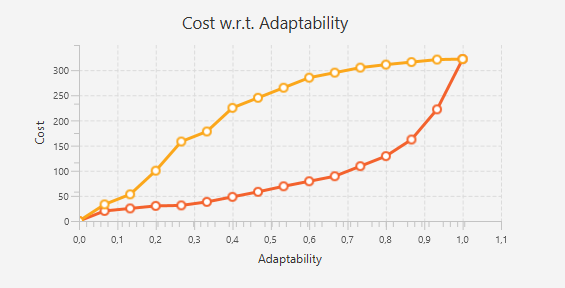
\includegraphics[scale=0.9]{img/generic-adapt.png}}
	\caption[Generic Generated Architecture Adaptability]{Generic Generated Architecture Adaptability.}
	\label{fig:generic-adapt}
\end{figure}
In the Adaptability figure is shown how big is the difference between the maximum and the minimum cost of the architecture even for the smallest levels of adaptability; with a more accurate analysis the software architect should understand that this happens because some components cost way more than others, in particular component \emph{C6-2}. Since the algorithm tries to provide as much services as possible these components impact a lot on the total cost of the architecture creating such a difference between the maximum and the minimum cost. 
\chapter{Future Works and Conclusions}
\label{cap:discussion}

This final chapter provides an overview of the possible future works
regarding process migration in HPC systems. Then, possible future developments of the
\texttt{mig} framework are suggested, including the extension to
iterative migration and InfiniBand. Finally, the current
limitations of the proposed approach are discussed along with
the conclusions of the overall work presented in this thesis.

\section{Enhancing process migration in HPC}
As depicted in Figure \ref{fig:cap7-scholar-mig}
the research interest in Process Migration targeting HPC systems
is still high and it has
a positive trend. This, in conjunction with the problematics described in
Chapter \ref{cap:introduction}, leads us to suppose that in the next years
the \emph{process migration} will become an hot research topic.

\begin{figure}[t]
		\centerline 
{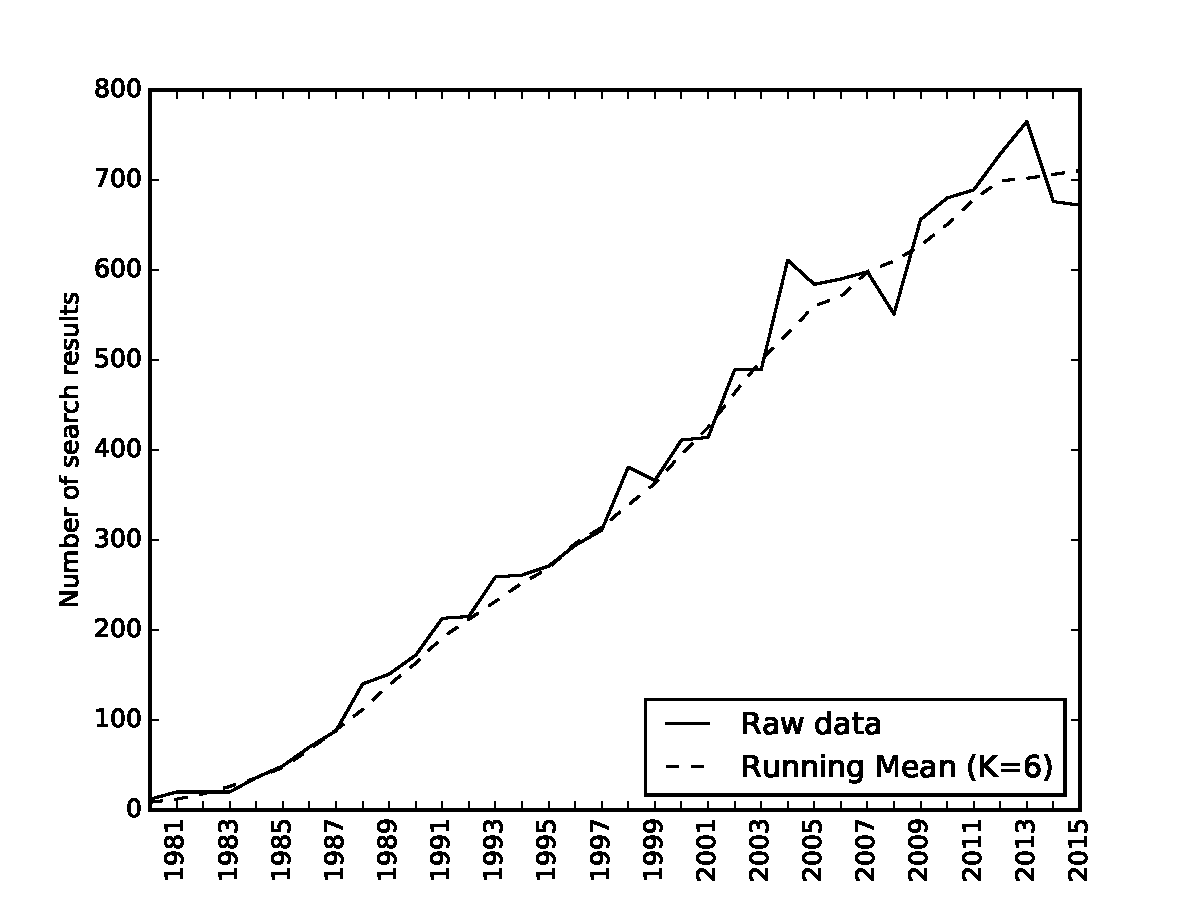
\includegraphics[scale=0.7]{img/cap7-scholar_mig}}
		\caption[Process migration trend in research]{Number of search results in Google Scholar with keyword
		"process migration"}
		\label{fig:cap7-scholar-mig}
\end{figure}


\subsection{Next challenges}
The CRIU project is rapidly evolving thanks to the very active development
community. Since the project is relatively young, it is still unstable,
especially for what concerns the advanced features. In the next years we
expect this project to reach a good level of maturity, such it could be used
also in production environments rather than only in research.

In parallel, new research challenges may arise and old issues may be addressed.
An example of such a case is the possibility managing process migration over
\textbf{heterogeneous processors}. The
explosion of several heterogeneous architectures, from the Graphical Processing
Units to specialized accelerators, requires the adoption of dedicated
techniques
in resource management and application frameworks. Therefore, low-level layer
capable of transparently move processes between processors or nodes with
different
architectures can become an essential feature. Unfortunately, this type of migration is
complex and implementing a working solution requires the involvement of several
computer engineering branches, from operating systems to compilers.
Previous research described in Chapter
\ref{cap:state-of-the-art} provided tools with strong limitations and that work
only for specific scenarios.

The first attempt that can be evaluated for an inclusion in CRIU is the
migration between general purpose architectures with different ISA 
(Instruction Set Architecture), for
instance to migrate a process between \texttt{x86\_64} and \texttt{AArch64}
architectures. The Checkpoint/Restart is already supported by CRIU for both architectures, but migrating processing between them is currently not possible. This because, such a type of migration
requires the translation of all the processors registers, the memory addresses
and other machine-dependent information. Moreover, since there is no one-to-one
correspondence between instructions with different ISA, some sort of
checkpoint barriers must be implemented in the binary code. To understand the
last problem consider the \texttt{MNEG} instruction of \texttt{ARMv8}
(\texttt{AArch64}) having this semantic: \( R_d = -R_n \cdot R_m\). This sort
of specialized instruction does not exist in \texttt{x86\_64} processors and
must be split into a multiplication and a subtraction. Consequently, a
migration mechanism cannot checkpoint the application between multiplication
and subtraction, thus it should consider an atomic operation both of them.
Managing this atomicity for different types of architecture seems not a
straightforward task and it necessarily requires additional support at compiler-level.

The previously described possible improvement in process migration may solve also
the problem of migrating processes between different Linux kernel versions or
different libraries, obviously provided that they expose the same API. As already
described in Chapter \ref{cap:design}, CRIU requires perfectly identical environments.

\subsection{Future developments}
The \texttt{mig} framework is not currently ready for production environments.
A sufficiently stable version has to be developed and possibly integrated
in the mainline repository of Open MPI. The stabilization of the \texttt{mig}
framework and related components requires extensive tests over different
environments and system setups. 

\subsubsection{Iterative Migration}
As we have seen, the transfer time dominates the migration time. This time
becomes an overhead in the overall application execution time, since the
processes
cannot progress during the image migration. However,
CRIU allows the \textbf{Iterative Migration} of processes: the processes
are checkpointed without killing them and, during the processes execution,
the image is transfered. As a result, the execution and image transfer time
are overlapped, this operation is often called \textbf{Pre-Copy}.
Obviously, the transfered image represents the
status of the application at the checkpoint time. Therefore, it does not
represent the current status of the migrating process and it must be updated
with the process memory and the context changes (register, etc.).

In HPC environment, the \emph{iterative migration} shows good performance
results, significantly lowering the migration overhead
\cite{wang2008proactive}. Therefore it can be considered a possible application
improvement to introduce in the \texttt{mig} framework, in order to limit the impact on the wall-time.

\subsubsection{InfiniBand}
The InfiniBand support is the prioritized task to be accomplished in the
development of \texttt{mig} framework. In HPC the InfiniBand networks are
very frequent, because their advantages compared to Ethernet.
InfiniBand presents lower overhead over Ethernet, because the applications are
able to directly communicate with the network adapter without the necessity
of operating system calls. Even considering the
10Gbit and 40Gbit Ethernet, InfiniBand FDR presents higher throughput and
lower latency compared with Ethernet protocols \cite{vienne2012performance}.
Furthermore, in 2014 the new InfiniBand EDR doubles the theoretical throughput
with respect to FDR.

Implementing the InfiniBand support should be a relatively easy task thanks 
to the high modularity of Open MPI. The
functions offered by the TCP \texttt{btl} component have to be replicated in
the InfiniBand \texttt{btl} component. The features provided by other modules -
like \texttt{mig} - are independents from the network protocol used.

\subsubsection{Removing the ORTE daemon granularity}
A further reduction of the \emph{ORTE daemon} overhead could be obtained by moving the
migration granularity to process-level, directly migrating MPI application
processes, instead of the underlying \emph{ORTE daemon}. This requires to change the
active BTL components of the migrating process. Whether \emph{process A} and
\emph{process B} are in the same node communicating via \emph{shared memory}
and
process B migrates towards another node, they have to change the active
\texttt{btl} component to a remote one (e.g. TCP or InfinBand) in order to
resume the connection to the other process. This change requires to address several
synchronization issues.

\subsection{Limitations}

The major limits of the proposed process migration mechanism are in similar
to those of the other C/R based systems: the nodes of HPC systems must be
homogeneous, i.e. the operating system (with kernel version), libraries version
and application binaries must be perfectly identical. Therefore, currently the
\texttt{mig} framework is not exploitable in heterogeneous environments.

Performing the checkpoint with CRIU requires administration
level permissions (\texttt{root} user in Linux) in all the nodes. This
limitation is a partial requirement of CRIU that is in progress to
be dropped by the CRIU development team. However, as previously
described, process migration requires the use of \texttt{unshare} system call,
that in turn requires the \texttt{CAP\_SYS\_ADMIN} capability in Linux. This
permission is usually granted only to the \texttt{root} user. Grant this
permission to non-administrative users may introduce security problems that
should be carefully evaluated and addressed.

In fault tolerant exploitation one of the most important issue to be addressed
is the possibility of migrating also the \emph{ORTE daemon} and
consequently the MPI processes from the HNP. Otherwise, the HNP becomes the
bottleneck in terms of fault-tolerance: the MTTF of the overall system is
reduced to the MTTF of the HNP. Since the \texttt{mpirun} command is actually
an \emph{ORTE daemon}, it would not be difficult to implement the migration of
HNP. We think the only needed change is the adaption of the coordination
protocol between \emph{ORTE daemons} and MPI processes.

\section{Conclusion}

In this thesis we introduced a novel approach to support process migration in
the Open MPI framework. The approach is based on handling the execution of
multiple \emph{ORTE daemon} instances, which can be thought of as the smallest
migratable unit. This is performed transparently to the application and the
non-involved Open MPI frameworks and components.

Compared to other state-of-the-art solutions, one of the major advantages
of our approach is the \emph{maintainability}. The extension introduced in the
Open MPI runtime in fact has a minimal impact on the other Open MPI frameworks.
Furthermore, on the application side the framework does not introduce any
additional API. Therefore its
exploitation it does not require any change on the applications code.

Moreover, the \texttt{mig} framework does not rely on any virtualization layer.
This constitutes a gain in terms of performance with respect to approaches
based
on virtual machine allocation. In this regard, our proposal allows us to
perform
fine-grained migrations, since the resource manager can decide between migrate
an entire application or a subset of its processes. This feature also
increases the controllability of the workload execution.

The integration with Barbeque Run-Time Resource Manager has been implemented
in order to exploit both Open MPI and the \texttt{mig} migration mechanism
in conjunction with a resource manager.
In this regard, a simple policy that solves an
Integer Linear Programming problem has been implemented as a BarbequeRTRM plugin.
This policy 
provides an optimal solution in most cases but it is
usable only with a small number of systems and applications. Therefore,
in the future a greedy policy must be implemented to work with large system,
in particular considering the Exascale computing horizon.

Through experimental tests, we shown how the overhead due to grouping the
application processes on top of several \emph{ORTE daemons} can be considered
negligible.
Conversely, stopping and resuming the processes execution on different nodes,
introduce an overhead dependent on the specific application, its input data
size, the network and the node capabilities.
As a consequence, a resource manager can play a key role to evaluate when a
migration is worth to be performed.

Overall, we can state that the work presented in this thesis is the first
process-level migration feature developed for Open MPI whose control is kept at
system-level (resource manager) and that does not require the code of
applications to be changed.

From the MPI communication standpoint, the lack of \emph{InfiniBand} support is
currently the most important missing feature. However the development of this
component is currently ongoing.

In next years, we can expect an increasing interest in process migration
and in general in C/R techniques. Therefore, the next steps of this work is to
sufficiently debug the code in order to add it to the Open MPI mainline
repository. In this way the \texttt{mig} framework may follow the rapid
developments of Open MPI and CRIU and it can be available for other resource
managers.


\appendix
\noappendicestocpagenum

\chapter{User Manual}
\label{app:usermanual}



\chapter{DistRib ILP formulation}
\label{app:distrib-ilp-formulation}
This appendix provides a formulation in \textbf{GNU MathProg} of the proposed
Integer Linear Programming problem used in the DistRib policy.

GNU MathProg is a high-level language to write mathematical models,
in particular optimization problems. It is specific to GLPK, but compatible
with the well-known \textbf{A Mathematical Programming Language (AMPL)}
\cite{fourer1990modeling}. To be precise, the GNU MathProf contains a subset
of instruction of the AMPL language.

The proposed formulation is implemented in BarbequeRTRM using the GLPK
libraries even if less intuitive than the GNU MathProg language. However, the
overhead drastically reduces, since a syntax parser of the model is not
required.

The GNU MathProg formulation is presented in Listing \ref{app2:mathprog}.

The proposed ILP has two variables, the \texttt{proc\_assigned} and the
\linebreak
\texttt{is\_assigned} variables
respectively correspond to the \(\pi\) and \(\phi\) of the mathematical
model presented in Chapter \ref{cap:integration}.

The parameters used in the formulation are:
\begin{itemize}
\item \texttt{num\_pe}: the vector containing the number of available 
processor elements per core.
\item \texttt{num\_proc}: the vector containing the number
of processes requested per application.
\item \texttt{priority}: the vector parameter
that represents \(p_a\), i.e. the priority for each application.
\item \texttt{sys\_penalty}: the vector parameter that represents \(r_s\),
i.e. an empirical number for per-system penalty.
\item \texttt{K\_dist}: the constant weight to the cost related to distribution
\item \texttt{max\_pe\_per\_system}: an arbitrarily number sufficient big to guarantee the constraints between \(\pi\) and \(\phi\) (details later).
\end{itemize}

After the definition of the cost objective function, there are four
constraints:
\begin{itemize}
\item \texttt{full\_assignment}: it assures that all the processes request of
each application is respected;
\item \texttt{resource\_availability}: it assures that the number of processes
assigned to each systems does not exceed the available processing elements;
\item \texttt{var\_association}: it bound the \(\pi\) and \(\phi\) variables in
sense that if \(\phi=1\) then  \(\pi \ge 1 \).

\item \texttt{var\_association\_rev}: the reverse bound between \(\pi\) and
\(\phi\), if \(\pi \ge 1\) then  \(\phi = 1 \).

\end{itemize}

\definecolor{britishracinggreen}{rgb}{0.0, 0.26, 0.15}
\lstdefinestyle{customc}{
  belowcaptionskip=1\baselineskip,
  breaklines=true,
  frame=L,
  xleftmargin=\parindent,
  language=C,
  showstringspaces=false,
  basicstyle=\footnotesize\ttfamily,
%  keywordstyle=\bfseries\color{green!40!black},
  commentstyle=\itshape\color{britishracinggreen},
  identifierstyle=\color{black},
  keywordstyle=\color{blue}\ttfamily,
  stringstyle=\color{orange},
alsoletter={.},
  morekeywords={%  
    set, var, in, integer, binary,param, minimize, sum, s.t.%
    }
}

\lstset{%
}%

\begin{figure}[t]
\begin{lstlisting}[style=customc]
set SYSTEMS;
set APPLICATIONS;

/* 
 * The only two necessary variables. The first one is not used in the cost
 * function but it's required for proper resource assignment.
 */
var proc_assigned{i in APPLICATIONS, j in SYSTEMS}, >=0, integer;
var is_assigned  {i in APPLICATIONS, j in SYSTEMS}, >=0, binary;

/* 
 * The various constant parameters.
 */
param num_pe     {j in SYSTEMS};
param num_proc   {i in APPLICATIONS};
param priority   {i in APPLICATIONS};
param sys_penalty{j in SYSTEMS};

param K_dist;
param max_pe_per_system; /* required for the constaints of binary variable,
                            it may be set to 1000000 or similar */

/* 
 * The minimization of the cost function.
 */
minimize cost: sum{i in APPLICATIONS} sum{j in SYSTEMS} 
                    ( priority[i] * 
                    (
                      proc_assigned[i,j] * sys_penalty[j]  + 
                      K_dist * is_assigned[i,j] 
                    ));

/* 
 * Constraints.
 */
s.t. full_assignment{i in APPLICATIONS}:
    sum{j in SYSTEMS} proc_assigned[i,j] >= num_proc[i,j];

s.t. resource_availability{j in SYSTEMS}:
    sum{i in APPLICATIONS} proc_assigned[i,j] <= num_pe[j];

s.t. var_association{i in APPLICATIONS, j in SYSTEMS}:
    is_assigned[i,j] <= proc_assigned[i,j];

s.t. var_association_rev{i in APPLICATIONS, j in SYSTEMS}:
    max_pe_per_system * is_assigned[i,j] >= proc_assigned[i,j];

\end{lstlisting}
\renewcommand\figurename{Listing}
\caption{The MathProg formulation of DistRib ILP solver.}
\label{app2:mathprog}
\end{figure}



\cleardoublepage
\phantomsection
\addcontentsline{toc}{chapter}{\bibname}
\small
\bibliographystyle{unsrt}
\bibliography{thesis}



\end{document}
